\documentclass[11pt,openany]{report}
\usepackage[letterpaper,margin=0.86in,headheight=15pt]{geometry}
\usepackage[T1]{fontenc}
\usepackage[utf8]{inputenc}
\usepackage{lmodern,microtype}
\usepackage{amsmath,amssymb,amsthm,mathtools}
\usepackage{booktabs,longtable,tabularx,array}
\usepackage{graphicx,float,enumitem,xcolor,fancyhdr}
\usepackage[hidelinks]{hyperref}
\usepackage{bookmark}
\definecolor{Ink}{HTML}{20303A}
\definecolor{Accent}{HTML}{226B66}
\definecolor{Muted}{HTML}{64747B}
\color{Ink}
\setlength{\parindent}{0pt}
\setlength{\parskip}{0.55em}
\setlength{\emergencystretch}{2em}
\raggedbottom
\allowdisplaybreaks
\newtheorem{theorem}{Theorem}[chapter]
\newtheorem{proposition}[theorem]{Proposition}
\newtheorem{lemma}[theorem]{Lemma}
\newtheorem{corollary}[theorem]{Corollary}
\theoremstyle{definition}
\newtheorem{definition}[theorem]{Definition}
\newtheorem{example}[theorem]{Example}
\theoremstyle{remark}
\newtheorem{remark}[theorem]{Remark}
\newcolumntype{L}[1]{>{\raggedright\arraybackslash}p{#1}}
\pagestyle{fancy}
\fancyhf{}
\fancyhead[L]{\small\color{Muted}Komorebi / Special Functions}
\fancyhead[R]{\small\color{Muted}Consolidated working edition}
\fancyfoot[C]{\small\thepage}
\renewcommand{\headrulewidth}{0.3pt}
\hypersetup{pdftitle={Komorebi Special Functions: Consolidated Manuscript v0.1},pdfauthor={Komorebi P.},pdfsubject={Packet realization, arithmetic resolvents, shape refinement, and recoupling}}

% Operation Komorebi: shared publication profile.
\usepackage{komorebi-publication}
\renewcommand{\KomorebiTitle}{Special Functions through Packet Realization}
\renewcommand{\KomorebiSubtitle}{A consolidated mathematical core: Projector Generated Special Functions I--VIII}
\renewcommand{\KomorebiSeries}{Research library}
\renewcommand{\KomorebiKind}{Traditional paper}
\renewcommand{\KomorebiEdition}{Working edition 0.1 / Standardized 8 October 2026}
\renewcommand{\KomorebiShortTitle}{Special Functions through Packet Realization}
\renewcommand{\KomorebiTitleSize}{31}
\renewcommand{\KomorebiTitleLeading}{36}
\renewcommand{\KomorebiProfile}{classical}
\renewcommand{\KomorebiOrientation}{portrait}
\KomorebiSetup
\begin{document}
\KomorebiCover

\hypersetup{pageanchor=false}

\pagenumbering{roman}
\hypersetup{pageanchor=true}
\chapter*{Editorial scope}
\addcontentsline{toc}{chapter}{Editorial scope}
This edition gives the eight special-function papers one mathematical entry point. It consolidates repeated definitions and theorem chains into three connected chapters, then supplies a selected visual atlas, a correction register, and an evidence map. The complete reader appends the eight original papers in order. Their original page numbers and statements remain visible, so the correction register must be read alongside them.

This is a first consolidated working edition. It is not a claim that all eight papers have undergone a new exhaustive proof audit or a complete Lean build. The mathematical chapters give concise proofs for elementary identities and explicitly distinguish source results, classical inputs, conditional extensions, and open arithmetic estimates. The correction register records the points exposed by the present bounded review.

The source package preserves the eight release archives, their code, tables, and figures. It also includes all 173 special-function records from the retrieved claim ledger, fresh test results, and the review notes. Claim records are provenance data. They are not interchangeable with Lean proof terms.

\textbf{Reading route.} Read Chapters 1--3 for the unified mathematics. Chapter 4 presents selected figures from the source papers. Chapters 5--6 identify corrections and the exact evidence scope. For full derivations and implementations, follow the source-volume references and the bookmarks in the complete reader.
\tableofcontents
\clearpage
\pagenumbering{arabic}
\chapter{An exact packet spine for special functions}

The first three volumes have a common mathematical spine: exact analysis and synthesis, refinement of an analytic seed, arithmetic scale transfer, a positive moment measure, and its spectral realizations. This chapter consolidates that spine while retaining the distinction between proved coordinate identities, classical asymptotic inputs, and the unresolved signed estimate. Source references name the original volume and claim title. They provide provenance rather than a new certification of every source proof.

\section{Coefficient packets and ordered differential transport}

Let $F(z)=\sum_{n\ge0}a_nz^n$ be an analytic germ at the origin and let $M\ge2$ be an integer. Its coefficient packets are
\[
F_{M,r}(u)=\sum_{m\ge0}a_{Mm+r}u^m,
\qquad 0\le r<M.
\]
These are analytic germs in $u$. This construction is Volume I, ``Residue-section functions'' and ``Exact polyphase reconstruction.''

\begin{proposition}[Exact packet reconstruction and refinement]
Where the defining series converge,
\[
F(z)=\sum_{r=0}^{M-1}z^rF_{M,r}(z^M).
\]
For an integer $L\ge1$, refinement satisfies
\[
F_{M,r}(u)=\sum_{\ell=0}^{L-1}u^\ell
F_{LM,r+M\ell}(u^L).
\]
\end{proposition}
\begin{proof}
The first identity partitions each exponent uniquely as $n=Mm+r$. In the second identity, partition the packet index as $m=Lj+\ell$. Then
$Mm+r=LMj+r+M\ell$, and the corresponding term is
$a_{LMj+r+M\ell}u^{Lj+\ell}$. Both identities preserve every coefficient.
\end{proof}

Write $\boldsymbol F_M=(F_{M,0},\ldots,F_{M,M-1})^T$. Define the carry matrix by
\[
C_M(u)_{0,M-1}=u,
\qquad C_M(u)_{r,r-1}=1\quad(1\le r<M),
\]
with all other entries zero, and define
\[
\Theta_M=Mu\frac{d}{du}I_M+
\operatorname{diag}(0,1,\ldots,M-1).
\]
The synthesis map $\mathcal S_M\boldsymbol f(z)=\sum_rz^rf_r(z^M)$ is injective on analytic packet germs. Multiplication and the Euler derivative intertwine as
\[
\mathcal S_M(C_M\boldsymbol f)=z\mathcal S_M\boldsymbol f,
\qquad
\mathcal S_M(\Theta_M\boldsymbol f)=
z\frac{d}{dz}\mathcal S_M\boldsymbol f.
\]
Indeed, multiplication advances the residue address and wraps the last address with one factor $u$; the Euler operator multiplies $u^m$ in address $r$ by $Mm+r$. Consequently
\[
[\Theta_M,C_M]=C_M.
\]
For every ordered polynomial differential expression $\mathcal L(z,\theta)$, where $\theta=z\,d/dz$,
\[
\mathcal L(z,\theta)F=0
\quad\Longrightarrow\quad
\mathcal L(C_M,\Theta_M)\boldsymbol F_M=0.
\]
Intertwine each ordered monomial and apply injectivity. This is Volume I, ``Intertwining laws,'' ``Weyl commutator,'' and ``Differential lift.'' The order of operator factors is part of the statement.

\section{Bernoulli--Hurwitz refinement}

For a real translation parameter $a>0$, define
\[
\mathfrak B(z;a)=-z\zeta(1-z,a),
\qquad
\mathfrak B_{M,r}(z;a)=
-zM^{z-1}\zeta\!\left(1-z,\frac{a+r}{M}\right).
\]
The order variable is $z\in\mathbb C$. The removable values are
$\mathfrak B(0;a)=1$ and $\mathfrak B_{M,r}(0;a)=1/M$.
The pole at $z=0$ is the only Hurwitz-zeta pole in this variable, so these functions are entire in $z$.

\begin{proposition}[Exact Bernoulli reconstruction and refinement]
For integers $M,L\ge1$ and $0\le r<M$,
\[
\mathfrak B(z;a)=\sum_{r=0}^{M-1}\mathfrak B_{M,r}(z;a),
\qquad
\mathfrak B_{M,r}(z;a)=
\sum_{\ell=0}^{L-1}\mathfrak B_{LM,r+\ell M}(z;a).
\]
For each positive integer $n$,
\[
\mathfrak B_{M,r}(n;a)=
M^{n-1}B_n\!\left(\frac{a+r}{M}\right).
\]
\end{proposition}
\begin{proof}
For $\operatorname{Re}s>1$, partition the Hurwitz series into residue classes to obtain
\[
\sum_{r=0}^{M-1}\zeta\!\left(s,\frac{a+r}{M}\right)
=M^s\zeta(s,a).
\]
Meromorphic continuation preserves this identity. Set $s=1-z$ and multiply by $-zM^{z-1}$. Apply the same identity to the children of a fixed parent to obtain refinement. The integer formula uses the classical special value $\zeta(1-n,x)=-B_n(x)/n$.
\end{proof}

These are Volume I, ``Reconstruction,'' ``Parent-child refinement,'' and ``Integer samples.'' Integer polynomial samples can also be evaluated at $a=0$, but the entire complex-order family above retains $a>0$.

Let $b_\ell=\mathfrak B_{LM,r+\ell M}(z;a)$ and $\omega_L=e^{2\pi i/L}$. The unitary child transform
\[
W_j=\frac1{\sqrt L}\sum_{\ell=0}^{L-1}
\omega_L^{-j\ell}b_\ell
\]
has the exact inverse $b_\ell=L^{-1/2}\sum_j\omega_L^{j\ell}W_j$ and preserves $\sum_\ell|b_\ell|^2$. Its DC channel is $W_0=\mathfrak B_{M,r}/\sqrt L$. Volume I derives the Lerch closed form, and Volume II derives the local Stieltjes expansion and scalar detail invariants from this same bank. These analytic invariants do not require the positive arithmetic measure introduced next.

\section{Signed arithmetic transfer and positive energy}

Let $q\ge1$ be an integer and $\chi$ a Dirichlet character modulo $q$. Throughout this section $\beta>0$ and $k$ is a nonnegative integer. At zero depth, use the moment convention $0^0=1$.

\begin{definition}[Arithmetic transfer and packet energy]
For $a>1$ and $t\in\mathbb R$, define the signed transfer
\[
C_{a,\beta,\chi}(k,t)=
\sum_{n\ge1}\frac{\mu(n)\chi(n)}{n^{a+it}}
(1-n^{-\beta})^k.
\]
For $a>1/2$, define the positive energy
\[
E_{a,\beta,q}(k)=
\sum_{\substack{n\ge1\\(n,q)=1}}
\frac{\mu(n)^2}{n^{2a}}(1-n^{-\beta})^{2k}.
\]
\end{definition}

The signed series is absolutely convergent in its stated range. The energy uses $|\chi(n)|^2=\boldsymbol 1_{(n,q)=1}$ and therefore depends on the modulus rather than the character values.

\begin{proposition}[Two exact finite-difference coordinates]
For $a>1$,
\[
C_{a,\beta,\chi}(k,t)=
\sum_{j=0}^{k}(-1)^j\binom{k}{j}
\frac1{L(a+\beta j+it,\chi)}.
\]
For $a>1/2$, set
\[
D_q(s)=\frac{\zeta(s)}{\zeta(2s)}
\prod_{p\mid q}(1+p^{-s})^{-1},\qquad \operatorname{Re}s>1.
\]
Then
\[
E_{a,\beta,q}(k)=
\sum_{j=0}^{2k}(-1)^j\binom{2k}{j}D_q(2a+\beta j).
\]
\end{proposition}
\begin{proof}
The absolutely convergent reciprocal Euler product gives
$L(s,\chi)^{-1}=\sum_n\mu(n)\chi(n)n^{-s}$.
The squarefree Dirichlet series has Euler factors $1+p^{-s}$ for $p\nmid q$, so it is $D_q(s)$. Expanding the corresponding powers of $1-n^{-\beta}$ and interchanging each finite sum with its absolutely convergent series proves both identities.
\end{proof}

The source claims are Volume I, ``M\"obius form,'' and Volume II, ``Exact zeta-ratio finite difference,'' repeated in Volume III. Their parallel form does not remove the arithmetic signs from $C$.

Put
\[
w_n=\mu(n)^2\boldsymbol 1_{(n,q)=1}n^{-2a},
\qquad x_n=(1-n^{-\beta})^2,
\qquad \nu=\sum_{n\ge1}w_n\delta_{x_n}.
\]
This is a finite positive measure, with atoms in $[0,1)$ and infinitely many distinct positive atoms. In particular the zero atom at $n=1$ is retained. Its moments satisfy $E_k=\int x^k\,d\nu(x)$.

\begin{proposition}[Positive moment and resolvent laws]
For $m,k\ge0$,
\[
(-1)^m\Delta^mE_k=\int x^k(1-x)^m\,d\nu(x)\ge0.
\]
Every finite Hankel matrix $(E_{i+j})_{0\le i,j\le d}$ is positive definite. The resolvent
\[
\mathcal E(z)=\int\frac{d\nu(x)}{1-zx}
\]
is analytic and zero-free on $\mathbb C\setminus[1,\infty)$, and for $|z|<1$ it equals $\sum_{k\ge0}E_kz^k$.
\end{proposition}
\begin{proof}
Finite differences act on $x^k$ by multiplication by $(x-1)^m$. For a nonzero coefficient vector $c$, the Hankel quadratic form is
\[
\int\left|\sum_{j=0}^dc_jx^j\right|^2d\nu(x)>0,
\]
because a nonzero polynomial cannot vanish at infinitely many distinct atoms. On every compact subset of the slit plane, $|1-zx|$ has a positive lower bound for $x\in[0,1]$, proving analyticity. For real $z<1$ the integrand is positive. For $\operatorname{Im}z>0$ its imaginary part is
\[
\frac{x\operatorname{Im}z}{|1-zx|^2},
\]
whose integral is strictly positive; the sign reverses below the real axis. A zero is impossible.
\end{proof}

These are Volume II, ``Complete monotonicity,'' ``Strict finite Hankel positivity,'' and ``Zero-free slit plane.'' Volume III further proves strict positivity of every generalized Hankel minor with strictly increasing nonnegative row and column exponents.

\section{Energy asymptotics and the all-moment bridge}

The classical squarefree counting input is
\[
\sum_{\substack{n\le X\\(n,q)=1}}\mu(n)^2
=\delta_qX+O_q(\sqrt X),
\qquad
\delta_q=\frac1{\zeta(2)}\prod_{p\mid q}\frac{p}{p+1}.
\]
The following asymptotic implication is the source result Volume II, ``Packet-energy asymptotic,'' also stated in Volumes I and III. It depends on that classical counting law.

\begin{proposition}[Source energy law]
Let $a>1/2$, $\beta>0$, and $\alpha=(2a-1)/\beta$. Then
\[
E_{a,\beta,q}(k)\sim
\frac{\delta_q}{\beta}\Gamma(\alpha)(2k)^{-\alpha}.
\]
\end{proposition}
\begin{proof}
The density part of Stieltjes summation is evaluated exactly by
\[
\delta_q\int_1^\infty x^{-2a}(1-x^{-\beta})^{2k}\,dx
=\frac{\delta_q}{\beta}\mathrm B(\alpha,2k+1).
\]
The counting remainder contributes at most a constant times
\[
\int_1^\infty\sqrt x
\left|\frac{d}{dx}\left[x^{-2a}(1-x^{-\beta})^{2k}\right]\right|dx
=O_{a,\beta,q}\left(k^{-(2a-1/2)/\beta}\right).
\]
This is lower order than $k^{-\alpha}$. The beta-function asymptotic gives the stated leading term. This records the source reduction to the classical counting input, rather than an independent re-audit of that input.
\end{proof}

For $k\ge1$, normalize the weights $w_nx_n^k/E_k$ into a probability law and put
\[
U_k=2k\,n^{-\beta},
\qquad
u_k=k(1-x_n)=U_k-\frac{U_k^2}{4k}.
\]
The first coordinate is Volume II's Gamma scaling coordinate, and the second is Volume III's endpoint coordinate.

\begin{proposition}[All-moment compatibility of the two coordinates]
For every nonnegative integer $m$,
\[
\mathbb E_k[U_k^m]
=(2k)^m\frac{E_{a+\beta m/2,\beta,q}(k)}{E_{a,\beta,q}(k)}
\longrightarrow\frac{\Gamma(\alpha+m)}{\Gamma(\alpha)}.
\]
The moments of $u_k$ have the same limits.
\end{proposition}
\begin{proof}
Multiplication by $n^{-\beta m}$ shifts the exponent $2a$ to $2a+\beta m$, proving the exact identity. Apply the source energy law to numerator and denominator. For $m\ge1$, $0\le u_k\le U_k$ and
\[
0\le U_k^m-u_k^m\le
\frac{m}{4k}U_k^{m+1}.
\]
The already proved $(m+1)$st moment convergence bounds the expectation on the right by $O(1/k)$. Thus every fixed moment transfers to the endpoint coordinate.
\end{proof}

These limits are the moments of $\operatorname{Gamma}(\alpha,1)$. The classical method of moments, using determinacy of the Gamma law, yields weak convergence as well. The all-moment conclusion is the required bridge to the polynomial and determinant results; bounded-test-function weak convergence alone would not supply it.

\section{Laguerre and finite spectral realizations}

Let $P_m^{(k)}$ be the monic orthogonal polynomial of degree $m$ for the law of $u_k$. Volume III, ``Fixed-degree Laguerre universality,'' identifies the limit
\[
P_m^{(k)}(u)\longrightarrow
(-1)^m m!L_m^{(\alpha-1)}(u)
\]
coefficientwise and locally uniformly for each fixed $m$. To see the implication, write orthogonality of
$u^m+\sum_{j<m}c_ju^j$ as a linear system in the first $2m$ moments. The limiting Gamma moment matrix is positive definite. The all-moment bridge and continuity of the inverse matrix therefore give convergence of the coefficients. The classical identification of Gamma orthogonal polynomials supplies the displayed Laguerre formula. Their squared monic norms under the normalized Gamma law are $m!(\alpha)_m$.

At fixed parameters, normalize $\nu$ by its mass $E_0$ and let $J_m$ be the leading $m\times m$ Jacobi matrix of its orthonormal polynomials. The classical Gaussian quadrature theorem gives the source result Volume III, ``Moment-exact packet reduction'': there are nodes $\xi_j\in(0,1)$ and positive weights $\lambda_j$ summing to one such that
\[
E_r=E_0\sum_{j=1}^m\lambda_j\xi_j^r
=E_0e_1^TJ_m^re_1,
\qquad 0\le r\le2m-1.
\]
The nodes belong to the interval spanned by the measure; they need not equal its discrete atoms. The reduced resolvent
\[
\mathcal E_m(z)=E_0\sum_{j=1}^m
\frac{\lambda_j}{1-z\xi_j}
\]
matches these first $2m$ Taylor coefficients and has poles on $(1,\infty)$. Its spectral weights are positive. In the $z$ coordinate, its residue at $z=1/\xi_j$ is $-E_0\lambda_j/\xi_j$.

Volume III develops the corresponding fixed-degree Jacobi, kernel, quadrature and shifted-Hankel limits. They depend on the all-moment implication above and classical orthogonal-polynomial identities. The principal cusp has a direct Abelian proof from the energy coefficients, supplied next.


\section{The principal cusp from the energy coefficients}

The following Abelian argument replaces the informal discrete-density passage
in Volume III, ``Principal edge cusp.'' It uses only the energy law already
stated above.

\begin{lemma}[An elementary square-root Abelian passage]
Let $c_k\ge0$ and $c_k\sim A k^{-3/2}$, where $A>0$. For
$F(z)=\sum_{k\ge0}c_kz^k$, one has $F(1)<\infty$ and
\[
F(1)-F(z)\sim2\sqrt\pi A\sqrt{1-z}
\qquad(z\uparrow1\text{ through real values}).
\]
\end{lemma}
\begin{proof}
Put $t=-\log z$ and
$S(t)=\sum_{k\ge1}k^{-3/2}(1-e^{-tk})$.
The function
\[
f(u)=u^{-3/2}(1-e^{-u})
=u^{-1/2}\int_0^1e^{-su}\,ds
\]
is positive and decreasing. It is integrable at both endpoints. Thus
\[
\int_t^\infty f(u)\,du
\le t\sum_{k\ge1}f(tk)
\le\int_0^\infty f(u)\,du=2\sqrt\pi,
\]
where integration by parts gives the last integral. Since
$\int_0^t f(u)du\le2\sqrt t$, it follows that
$S(t)=2\sqrt\pi\sqrt t+O(t)$.

Write $r_k=c_k-Ak^{-3/2}$ for $k\ge1$. For each $\varepsilon>0$, choose $K$
such that $|r_k|\le\varepsilon k^{-3/2}$ for $k\ge K$. Then
\[
|F(1)-F(e^{-t})-AS(t)|
\le t\sum_{1\le k<K}k|r_k|+\varepsilon S(t).
\]
Divide by $\sqrt t$, let $t\downarrow0$, and then let $\varepsilon\downarrow0$.
Finally, $t\sim1-z$. The coefficient hypothesis also guarantees summability.
\end{proof}

For the principal energy $a=\beta=2$, $q=1$, the coefficient law gives
$A=3/(2^{5/2}\pi^{3/2})$. Therefore the source cusp is
\[
\mathcal E(1)-\mathcal E(z)
\sim\frac{3}{2^{3/2}\pi}\sqrt{1-z}.
\]
This proof supplies the missing local implication. The actual coefficient
asymptotic warrants an $o(\sqrt{1-z})$ remainder; it does not by itself supply
an $O(1-z)$ remainder. The Abelian lemma received a separate neutral review
in this consolidation, conditional on the source energy asymptotic.

\section{The remaining signed arithmetic estimate}

For the principal parameters $a=\beta=2$ and $q=1$, write
\[
c_k=\sum_{n\ge1}\frac{\mu(n)}{n^2}(1-n^{-2})^k,
\qquad
E_k=\sum_{n\ge1}\frac{\mu(n)^2}{n^4}(1-n^{-2})^{2k}.
\]
The positive theory gives
\[
E_k\sim\frac{3}{2^{5/2}\pi^{3/2}}k^{-3/2}.
\]
The classical B\'aez-Duarte theorem (Theorem 1.1, 2005, checked in the published source) is the external input
\[
\mathrm{RH}\quad\Longleftrightarrow\quad
c_k=O_\varepsilon(k^{-3/4+\varepsilon})
\quad\text{for every }\varepsilon>0.
\]
It is cited in Volume I, ``Coherence form of the B\'aez-Duarte criterion,'' and Volume II, ``Normalized principal coherence criterion.'' Consequently, defining $\Gamma_k=|c_k|^2/E_k$,
\[
\mathrm{RH}\quad\Longleftrightarrow\quad
\Gamma_k=O_\varepsilon(k^\varepsilon)
\quad\text{for every }\varepsilon>0.
\]
Indeed, square the amplitude bound and divide by the energy law; in the reverse direction multiply by the energy law and take square roots. The arbitrary positive exponent can be renamed in either direction.

This is an equivalence with an open arithmetic estimate. The positive moment measure determines the normalization and supports exact finite models. The estimate still concerns cancellation of the signs $\mu(n)$ inside the principal transfer. Volume II's cross-character decoherence concerns a different Gram entry with coefficients $\mu(n)^2\chi(n)\overline{\psi(n)}$ for distinct characters modulo one fixed modulus. Its cancellation theorem does not estimate $c_k$.

The common construction therefore separates three achievements precisely: exact packet identities, positive spectral and scaling laws, and a signed coherence target whose truth is equivalent to RH. Consolidation preserves all three without treating the third as a consequence of the first two.

\chapter{From arithmetic depth to a Gamma shape calculus}
\label{chap:shape-core}

Volumes IV--VI follow one continuous
route. A signed number-basis amplitude has a positive time-averaged Gram
kernel. Large depth fixes the shape and centering of a log-Gamma window. Exact
transforms of that window then produce a phase-space kernel, orthogonal
polynomial coordinates, shape refinement, and coherent smoothing. This chapter
introduces the shared objects once. Source references identify the original
volume and claim title. Elementary identities are rederived here. The
arithmetic asymptotic and classical orthogonal-polynomial inputs retain their
original hypotheses and evidence scope.

\section{The arithmetic seed and its positive lift}

Retain Chapter 1's signed transfer $C_{a,\beta,\chi}(k,t)$, with
$\beta>0$, $a>1$, and $\chi$ modulo $q$. Put $d_n=1-n^{-\beta}$.
The zero-depth convention retains $n=1$. We now add a two-depth positive kernel.
The positive companion is defined already for $a>1/2$:
\[
 \mathcal K_q(k,\ell;\tau)
 =\sum_{\substack{n\geq1\\(n,q)=1}}
 \mu(n)^2 n^{-2a-i\tau}d_n^{k+\ell}.
\]

\begin{proposition}[Time-average Gram lift]
For $a>1$, the long-time cross-correlation satisfies
\[
 \lim_{T\to\infty}\frac1{2T}\int_{-T}^{T}
 C_{a,\beta,\chi}(k,t+\tau)\overline{C_{a,\beta,\chi}(\ell,t)}\,dt
 =\mathcal K_q(k,\ell;\tau).
\]
For $a>1/2$, the kernel
$\mathcal K_q(k,\ell;t-s)$ is positive definite on depth-time pairs.
\end{proposition}

\begin{proof}
Absolute convergence for $a>1$ permits expansion of the correlation into a
double series and passage through the time average. A term with indices $n,m$
contains $e^{-it(\log n-\log m)}$. Its mean is one for $n=m$ and tends to zero
otherwise. This leaves the displayed squarefree diagonal.
For positivity, set
$v_{k,t}(n)=\mu(n)\chi(n)n^{-a}d_n^k n^{-it}$.
These vectors are square summable for $a>1/2$, and the kernel is
$\sum_n v_{k,t}(n)\overline{v_{\ell,s}(n)}$.
Every finite kernel matrix is a Gram matrix.
\end{proof}

This is Paper IV, ``Exact time-average identity'' and ``Positive-definite packet
kernel.'' Time averaging retains the positive diagonal power and removes the
off-diagonal frequency interference. It does not bound the original signed
amplitude at a particular time.

Define
\[
 \alpha=\frac{2a-1}{\beta},\qquad
 \delta_q=\frac1{\zeta(2)}\prod_{p\mid q}\frac{p}{p+1}.
\]
The fixed-modulus squarefree counting input is
$\sum_{n\leq X,(n,q)=1}\mu(n)^2=\delta_q X+O_q(X^{1/2})$.
Paper IV, ``Uniform complex packet asymptotic,'' uses partial summation to obtain
\[
 \mathcal K_q(k,\ell;\tau)
 \sim\frac{\delta_q}{\beta}\Gamma(\alpha+i\tau/\beta)
 (k+\ell)^{-\alpha-i\tau/\beta}.
\]
Paper V, ``Joint arithmetic phase-space limit,'' combines the diagonal
normalizations. Uniformly when $k/\ell$ stays in a compact subset of
$(0,\infty)$ and $\tau$ stays in a compact real interval, with
$h=\log(k/\ell)$ and $\eta=\tau/\beta$,
\begin{equation}
 e^{i\eta\log(2\sqrt{k\ell})}
 \frac{\mathcal K_q(k,\ell;\tau)}
 {\sqrt{\mathcal K_q(k,k;0)\mathcal K_q(\ell,\ell;0)}}
 \longrightarrow
 \frac{\Gamma(\alpha+i\eta)}{\Gamma(\alpha)}
 \operatorname{sech}^{\alpha+i\eta}(h/2).
 \label{eq:shape-arithmetic-limit}
\end{equation}
The positive domain is $a>1/2$. The signed series above and its absolute
time-average derivation use the stronger condition $a>1$.

\section{One window and its exact phase-space kernel}

For an independent shape $\alpha>0$, define
\[
 g_\alpha(y)=\Gamma(\alpha)^{-1/2}
 \exp\left(\frac{\alpha y}{2}-\frac{e^y}{2}\right),
 \qquad y\in\mathbb R.
\]
The substitution $u=e^y$ gives
$\int |g_\alpha|^2dy=\Gamma(\alpha)^{-1}
\int_0^\infty u^{\alpha-1}e^{-u}du=1$.
Thus $|g_\alpha|^2$ is a log-Gamma density. Its shape is fixed by the arithmetic
limit in \eqref{eq:shape-arithmetic-limit}, but the exact window theory makes
sense for every positive shape.

Use a second shape $\gamma$ to distinguish shape composition from the arithmetic
scale exponent. The centered cross-ambiguity convention is
\[
 A_{\alpha,\gamma}(h,\eta)
 =\int_{\mathbb R}g_\alpha(y+h/2)g_\gamma(y-h/2)e^{i\eta y}\,dy.
\]

\begin{theorem}[Cross-shape Gamma--sech identity]
For $\alpha,\gamma>0$ and real $h,\eta$, with $\lambda=(\alpha+\gamma)/2$,
\begin{equation}
 A_{\alpha,\gamma}(h,\eta)
 =e^{(\alpha-\gamma)h/4}
 \frac{\Gamma(\lambda+i\eta)}{\sqrt{\Gamma(\alpha)\Gamma(\gamma)}}
 \operatorname{sech}^{\lambda+i\eta}(h/2).
 \label{eq:shape-cross-ambiguity}
\end{equation}
\end{theorem}

\begin{proof}
Multiplication of the shifted windows leaves the constant prefactor
$e^{(\alpha-\gamma)h/4}/\sqrt{\Gamma(\alpha)\Gamma(\gamma)}$
and the integrand
$\exp((\lambda+i\eta)y-e^y\cosh(h/2))$.
The substitution $u=e^y\cosh(h/2)$ evaluates the remaining integral as
$\Gamma(\lambda+i\eta)\cosh^{-\lambda-i\eta}(h/2)$.
\end{proof}

This is Paper VI, ``Cross-shape Gamma--sech formula.'' At equal shapes it is
Paper V, ``Exact ambiguity formula,'' and precisely the arithmetic limit.
The Gamma function has no zeros and $\cosh(h/2)>0$ on the real line, so this
cross-ambiguity is nonzero on real phase space. At $h=\eta=0$ its value is
\[
 F(\alpha,\gamma)=
 \frac{\Gamma((\alpha+\gamma)/2)}{\sqrt{\Gamma(\alpha)\Gamma(\gamma)}}.
\]
Cauchy--Schwarz gives $0<F\leq1$, with equality only for equal shapes.
Indeed, the ratio of the two positive windows is a constant times
$e^{(\alpha-\gamma)y/2}$ and can be constant only when $\alpha=\gamma$.

\section{Fourier density and additive shape}

Under the unitary convention
$\widehat f(\omega)=(2\pi)^{-1/2}\int f(y)e^{-i\omega y}dy$, the same
Gamma integral gives
\[
 \widehat g_\alpha(\omega)=
 \frac{2^{\alpha/2-i\omega}\Gamma(\alpha/2-i\omega)}
 {\sqrt{2\pi\Gamma(\alpha)}}.
\]
Its squared modulus is the symmetric Meixner density
\[
 \rho_\alpha(\omega)=
 \frac{2^{\alpha-1}}{\pi\Gamma(\alpha)}
 |\Gamma(\alpha/2+i\omega)|^2.
\]
The Fourier autocorrelation identity and the zero-modulation ambiguity slice
give
\[
 \int_{\mathbb R}\rho_\alpha(\omega)e^{ih\omega}d\omega
 =\operatorname{sech}^{\alpha}(h/2).
\]
Consequently Fourier uniqueness proves the shape convolution law
\[
 \rho_{s+t}=\rho_s*\rho_t,\qquad s,t>0.
\]
These are Paper V, ``Fourier transform of the log-Gamma packet'' and ``Exact
characteristic function,'' followed by Paper VI, ``Meixner shape semigroup.''

The cross-ambiguity energy also separates exactly:
\begin{equation}
 \frac{|A_{\alpha,\gamma}(h,\eta)|^2}{2\pi}
 =p_{\alpha,\gamma}(h)\rho_{\alpha+\gamma}(\eta),
 \qquad
 p_{\alpha,\gamma}(h)=
 \frac{\Gamma(\alpha+\gamma)e^{(\alpha-\gamma)h/2}}
 {2^{\alpha+\gamma}\Gamma(\alpha)\Gamma(\gamma)}
 \operatorname{sech}^{\alpha+\gamma}(h/2).
 \label{eq:shape-factorization}
\end{equation}
Direct cancellation of constants proves the formula. Setting
$u=e^h/(1+e^h)$ transforms $p_{\alpha,\gamma}(h)dh$ into the
Beta$(\alpha,\gamma)$ probability law. Both factors are normalized. This is
Paper VI, ``Exact cross-spectrogram factorization.''

\section{Polynomial refinement and the common ladder}

The classical Meixner--Pollaczek polynomial input is specified by its generating
function, rather than by an implicit choice of sign or phase:
\[
 \sum_{n\geq0}P_{n,s}(x)z^n
 =(1-iz)^{-s/2+ix}(1+iz)^{-s/2-ix},\qquad |z|<1.
\]
Let $(s)_n=\Gamma(s+n)/\Gamma(s)$ and put
\[
 p_{n,s}(x)=\sqrt{\frac{n!}{(s)_n}}P_{n,s}(x).
\]
Classical orthogonality makes these a normalized polynomial basis in
$L^2(\rho_s(x)dx)$. The degree $n$ and shape $s$ are separate coordinates.

\begin{theorem}[Normalized two-child refinement]
For $\alpha,\gamma>0$,
\[
 p_{n,\alpha+\gamma}(x+y)
 =\sum_{r=0}^{n}
 \sqrt{\binom nr\frac{(\alpha)_r(\gamma)_{n-r}}
 {(\alpha+\gamma)_n}}
 p_{r,\alpha}(x)p_{n-r,\gamma}(y).
\]
The squared coefficients sum to one.
\end{theorem}

\begin{proof}
Multiplying the generating functions with shapes $\alpha,\gamma$ produces the
one with shape $\alpha+\gamma$ and argument $x+y$. Coefficient comparison gives
the unnormalized addition formula, and the displayed normalizations give the
square roots. The coefficient identity
$\sum_r\binom nr(\alpha)_r(\gamma)_{n-r}=(\alpha+\gamma)_n$
follows by comparing coefficients in
$(1-z)^{-\alpha}(1-z)^{-\gamma}=(1-z)^{-\alpha-\gamma}$.
\end{proof}

Paper VI, ``Two-child packet refinement,'' interprets the coefficient squares
as a beta-binomial law. For many children they become the
Dirichlet-multinomial coefficients
\[
 C_{n,\mathbf r}^{\mathbf s}
 =\sqrt{\frac{n!\prod_j(s_j)_{r_j}}
 {(\sum_js_j)_n\prod_jr_j!}},\qquad \sum_jr_j=n.
\]
Multiplication of generating functions proves this extension. Intermediate
Pochhammer factors cancel along every binary refinement tree, establishing the
coassociativity recorded in Paper VI.

There is a complementary position basis. Classical Laguerre orthogonality gives
\[
 L_{n,\alpha}^{\mathrm{packet}}(y)
 =\sqrt{\frac{n!}{\Gamma(n+\alpha)}}
 e^{\alpha y/2-e^y/2}L_n^{(\alpha-1)}(e^y).
\]
Paper V, ``Laguerre--Meixner Fourier duality,'' evaluates its transform as
\[
 \widehat{L_{n,\alpha}^{\mathrm{packet}}}(\omega)
 =i^n\widehat g_\alpha(\omega)p_{n,\alpha}(\omega).
\]
The phase $i^n$ is part of the identity. The polynomial frequency basis and the
Fourier-transformed position basis therefore differ by degree-dependent phases.

On an abstract orthonormal basis $e_n$, define
\[
 K_0e_n=(n+\alpha/2)e_n,\quad
 K_+e_n=\sqrt{(n+1)(n+\alpha)}e_{n+1},\quad
 K_-e_n=\sqrt{n(n+\alpha-1)}e_{n-1}.
\]
On its finite linear span, direct calculation gives
\[
 [K_0,K_+]=K_+,\quad [K_0,K_-]=-K_-,\quad
 [K_-,K_+]=2K_0,
\]
and the Casimir is $\frac\alpha2(\frac\alpha2-1)I$.
The Laguerre multiplication recurrence has matrix
$2K_0-K_+-K_-$; the real polynomial Meixner frequency recurrence has matrix
$(K_++K_-)/2$. These are two coordinate realizations of one ladder. A Fourier
comparison must retain the degree phases above. This is Paper V,
``$\mathfrak{su}(1,1)$ relations.''

\section{Shape transfer and its exact contraction spectrum}

Let $X_s$ have law $\rho_s$ and let $Y_t$ be an independent increment with law
$\rho_t$. Shape convolution gives $X_s+Y_t\sim\rho_{s+t}$. Conditioning the
refinement identity on $X_s$ removes all positive-degree increment polynomials
by orthogonality. Thus
\[
 \mathbb E[p_{n,s+t}(X_s+Y_t)\mid X_s]
 =\sigma_n(s,t)p_{n,s}(X_s),\qquad
 \sigma_n(s,t)=\sqrt{\frac{(s)_n}{(s+t)_n}}.
\]
For the transfer
$T_{s,t}:L^2(\rho_{s+t})\to L^2(\rho_s)$ given by
$T_{s,t}f(x)=\int f(x+y)\rho_t(y)dy$, these are its singular values in the
classical complete polynomial bases. They satisfy
\[
 \sigma_n(s,t)\sigma_n(s+t,u)=\sigma_n(s,t+u),\qquad
 \sigma_n(s,t)\sim
 \sqrt{\frac{\Gamma(s+t)}{\Gamma(s)}}n^{-t/2}.
\]
The transfer is compact for every $t>0$ and belongs to $S_p$ precisely when
$pt>2$. Its mean-zero operator norm is $\sqrt{s/(s+t)}$. These are Paper VI,
``Polynomial martingale law'' and ``Cocycle and compactness.'' The completeness
input matters for a statement about the entire operator, rather than only its
polynomial restriction.

\section{Coherent smoothing and its Gaussian limit}

Take the inner product conjugate-linear in its first argument. The centered
Weyl states are
\[
 \psi_{\alpha,u,\eta}(y)=e^{i\eta(y-u/2)}g_\alpha(y-u).
\]
Their exact overlap is
\[
 \langle\psi_{\alpha,u,\eta},\psi_{\gamma,v,\nu}\rangle
 =e^{i(\nu u-\eta v)/2}A_{\alpha,\gamma}(v-u,\nu-\eta).
\]
The Moyal identity for the normalized window gives the continuous tight frame
\[
 \frac1{2\pi}\int_{\mathbb R^2}
 |\langle\psi_{\alpha,u,\eta},f\rangle|^2du\,d\eta=\|f\|_2^2.
\]
Its coherent transform has a reproducing kernel equal to this overlap.
These are Paper VI, ``Cross-shape coherent overlap'' and ``Continuous tight
frame.''

The lower symbol of the associated anti-Wick operator is convolution with
\[
 B_\alpha(h,\eta)=\frac{|A_{\alpha,\alpha}(h,\eta)|^2}{2\pi}
 =p_\alpha(h)\rho_{2\alpha}(\eta),\qquad
 p_\alpha(h)=\frac{\Gamma(\alpha+1/2)}{2\sqrt\pi\Gamma(\alpha)}
 \operatorname{sech}^{2\alpha}(h/2).
\]
Its ordinary two-dimensional Fourier multiplier is
\[
 \widehat B_\alpha(\xi,x)
 =\frac{|\Gamma(\alpha+i\xi)|^2}{\Gamma(\alpha)^2}
 \operatorname{sech}^{2\alpha}(x/2).
\]
It is strictly positive on real dual space and tends to zero at infinity.
Therefore the Berezin convolution is injective on $L^2$ but has an unbounded
inverse on its range, as Paper VI states in ``Injectivity and ill-posed
inversion.'' Exact recoverability is not a stability bound.

For independent $H_\alpha\sim p_\alpha$ and
$\Omega_\alpha\sim\rho_{2\alpha}$, the standardized variables
\[
 Z_\alpha=\sqrt{\alpha/2}\,H_\alpha,\qquad
 W_\alpha=\sqrt{2/\alpha}\,\Omega_\alpha
\]
converge to independent standard Gaussians. For position this follows from the
Gamma-ratio characteristic function with argument
$\xi\sqrt{\alpha/2}$; for frequency it follows from
$\operatorname{sech}^{2\alpha}(x/\sqrt{2\alpha})\to e^{-x^2/2}$.
Paper VI, ``Gaussian marginal limits,'' proves this distributional limit.
Its stronger ``Heat-operator limit'' also uses controlled moments and
multiplier derivatives to assert Schwartz-seminorm convergence of the
rescaled convolution to $e^{\Delta/2}$. That stronger source claim is not
inferred here solely from convergence in distribution or a finite-grid plot.

\section{The signed branch and its retained boundary}

The positive shape calculus does not replace the signed arithmetic problem.
For $a>1$ the signed generating function is
\[
 \mathcal C_{a,\beta,\chi}(z,t)
 =\sum_{n\geq1}\frac{\mu(n)\chi(n)n^{-a-it}}{1-z(1-n^{-\beta})}.
\]
Paper IV continues it off the physical cut and proves
\[
 (1-z)\mathcal C_{a,\beta,\chi}(z,t)
 +z\mathcal C_{a+\beta,\beta,\chi}(z,t)=L(a+it,\chi)^{-1}.
\]
Its nonzero Hankel determinant supplies a unique rational Pad\'e matching
function with degree bounds $\deg P\leq m-1$, $\deg Q\leq m$ and
$Q(0)=1$, preserving the first $2m$ Taylor coefficients. An ordinary
$m$-term simple-packet decomposition additionally follows when $\deg Q=m$
and $Q$ has $m$ simple zeros. This chapter makes no universal claim of full
denominator degree, nonbreakdown, physical-interval signed nodes, or stable
inversion.

The principal signed coherence target and its exact RH equivalence are
stated once in Chapter 1. The shape windows, convolution laws, refinement
coefficients, and coherent frames provide positive structure; that open target
still concerns cancellation of the original M\"obius signs.

\chapter{Recoupling packets and their q-deformation}

The recoupling papers share one mathematical chain: a tensor excitation space is reduced to a lowest-weight multiplicity space, intermediate Casimirs select coordinate atlases, and their overlap supplies both reversible amplitudes and a measured stochastic channel. Four-factor tree atlases add a loop identity, and every finite overlap admits a rotation compiler. This chapter presents that chain once, with the ordinary theory as the specialization $q=1$.

The direct finite identities are separated from the classical representation-theoretic inputs. The name Racah records the classical identification of a recoupling matrix. An explicit comparison with a scalar polynomial requires additional parameter, normalization, and phase data.

\section{A single ladder and coproduct convention}

The ordinary ladder in Chapter 2 is recovered with $\kappa=\alpha/2$ and $q=1$. In this chapter, $q$ denotes the real deformation coordinate rather than the integer character modulus of Chapters 1--2. Let $0<q\leq1$ and let every shape $\kappa_r$ be positive. Define
\[
[x]_q=\frac{q^x-q^{-x}}{q-q^{-1}}\quad(q\ne1),
\qquad [x]_1=x.
\]
Equivalently, for $q=e^{-\theta}$, $[x]_q=\sinh(x\theta)/\sinh\theta$. In particular, $[x]_q>0$ for $x>0$.

\begin{definition}[Positive shape ladder]
On the algebraic finite-support span of an orthonormal basis $\{|n\rangle:n\geq0\}$, set
\[
K_0|n\rangle=(n+\kappa)|n\rangle,
\]
\[
K_+|n\rangle=\sqrt{[n+1]_q[2\kappa+n]_q}|n+1\rangle,
\qquad
K_-|n\rangle=\sqrt{[n]_q[2\kappa+n-1]_q}|n-1\rangle,
\]
where $K_-|0\rangle=0$. Tensor factors retain their declared order. Their coproduct is
\[
\Delta K_0=K_0\otimes I+I\otimes K_0,
\qquad
\Delta K_\pm=K_\pm\otimes q^{K_0}+q^{-K_0}\otimes K_\pm.
\]
\end{definition}

\noindent\emph{Source: VII, ``Positive shape packet''; VIII, ``Local q-algebra'' and ``Coassociative packet routing.'' Evidence: direct algebraic identities.}

The ladder obeys $[K_0,K_\pm]=\pm K_\pm$ and $[K_-,K_+]=[2K_0]_q$. The second identity follows from
\[
[x+1]_q[y]_q-[x]_q[y-1]_q=[x+y]_q.
\]
The coproduct preserves these relations: the mixed commutators cancel using $q^{K_0}K_\pm q^{-K_0}=q^{\pm1}K_\pm$, and the diagonal terms use $[x+y]_q=[x]_q q^y+q^{-x}[y]_q$. Since $q^{\Delta K_0}=q^{K_0}\otimes q^{K_0}$, either order of a three-factor iteration gives
\[
K_\pm\otimes q^{K_0}\otimes q^{K_0}
+q^{-K_0}\otimes K_\pm\otimes q^{K_0}
+q^{-K_0}\otimes q^{-K_0}\otimes K_\pm.
\]
Thus the displayed routing is coassociative.

The Casimir is
\[
C_q=[K_0]_q[K_0-1]_q-K_+K_-.
\]
Direct substitution on $|n\rangle$ yields $C_q=[\kappa]_q[\kappa-1]_q I$. The identity $[x+1]_q[x]_q-[x]_q[x-1]_q=[2x]_q$ also shows that $C_q$ commutes with the ladder generators. For an intermediate contiguous tensor block, this centrality supplies a real symmetric block Casimir commuting with the total lowering map. Contiguous blocks are sufficient for every planar tree used below.

\section{Excitation reduction and the two-factor seed}

For $m\geq2$ ordered factors and $N\geq0$, define
\[
H_N^{(m)}=\operatorname{span}\{|n_1,\ldots,n_m\rangle:\textstyle\sum_r n_r=N\},
\qquad
M_N^{(m)}=\ker(K_-^{[m]}|_{H_N^{(m)}}).
\]
These are finite spaces even though the local ladders are infinite.

\begin{proposition}[Multiplicity dimension]
\[
\dim H_N^{(m)}=\binom{N+m-1}{m-1},
\qquad
\dim M_N^{(m)}=\binom{N+m-2}{m-2}.
\]
\end{proposition}

\begin{proof}
The first count is the weak-composition count. For $N>0$, associate to each target composition $t$ of $N-1$ the source $t+e_m$. Its last-factor lowering coefficient is nonzero. Every earlier-factor lowering from that source has a larger last coordinate than $t$. Ordering by this coordinate gives a triangular square submatrix with nonzero diagonal. The lowering map is onto, and rank-nullity gives the second count. At $N=0$, the lowering map has zero target and both dimensions are one.
\end{proof}

\noindent\emph{Source: VII, ``Multiplicity dimension''; VIII, ``Multiplicity dimension.'' Evidence: direct finite proof, using VIII's explicit rank argument.}

Let $Q_N$ be an orthonormal frame for $M_N^{(m)}$. A Casimir acting on a contiguous intermediate block restricts to $Q_N^{\mathsf T}C_AQ_N$. The ratio of full to reduced dimension is $(N+m-1)/(m-1)$. This is an exact dimensional reduction. It does not assert a universal floating-point accuracy or runtime bound.

The two-factor kernel has dimension one. For $|\Omega_N\rangle=\sum_{n=0}^N c_n|n,N-n\rangle$, the lowering equation gives
\[
\frac{c_{n+1}}{c_n}
=-q^{-(N-1+\kappa_1+\kappa_2)}
\sqrt{\frac{[N-n]_q[2\kappa_2+N-n-1]_q}
{[n+1]_q[2\kappa_1+n]_q}}.
\]
For example, writing $\lambda=q^{-(N-1+\kappa_1+\kappa_2)}$, a normalized solution is
\[
c_n=Z_N^{-1/2}(-\lambda)^n
\sqrt{\frac{[N]_q!}{[n]_q![N-n]_q!}
\frac{\prod_{r=0}^{n-1}[2\kappa_2+N-n+r]_q}
{\prod_{r=0}^{n-1}[2\kappa_1+r]_q}}.
\]
Here empty products and $[0]_q!$ are one, and $Z_N$ is the positive sum of the displayed squared unnormalized coefficients. The ratio proves the formula. The scalar q-Hahn identification of general coupled coefficients is a classical representation-theoretic input.

\noindent\emph{Source: VIII, ``Explicit q-Hahn lowest packet.'' Evidence: direct finite recurrence and normalization.}

\section{Atlases, recoupling, and recurrence gauges}

For three factors, $\dim M_N^{(3)}=N+1$. Choose orthonormal eigenbases $L_N$ and $R_N$ of the restricted pair Casimirs $C_{12}$ and $C_{23}$, with columns expressed in the same multiplicity frame. Define the signed overlap
\[
\mathcal R_N=L_N^{\mathsf T}R_N.
\]

\begin{theorem}[Finite reconstruction]
\[
\mathcal R_N^{\mathsf T}\mathcal R_N
=\mathcal R_N\mathcal R_N^{\mathsf T}=I_{N+1}.
\]
Consequently, either atlas analyzes and synthesizes every vector in the same multiplicity space exactly.
\end{theorem}

\begin{proof}
Both basis matrices are orthogonal in the common frame. Multiplying their overlap and its transpose gives the identity.
\end{proof}

\noindent\emph{Source: VII, ``Perfect recoupling reconstruction''; VIII, ``Exact analysis and synthesis.'' Evidence: direct linear algebra.}

The usual positive-series decomposition gives the intermediate pair eigenvalues
\[
\lambda_j^{ab}=[\kappa_a+\kappa_b+j]_q
[\kappa_a+\kappa_b+j-1]_q,\qquad 0\leq j\leq N.
\]
Their occurrence and the Racah/q-Racah identification are classical representation-theoretic inputs cited by VII and VIII. The release reconstructs the matrices and checks their spectra in bounded examples. It does not supply the full scalar parameter and normalization map in the symmetric q convention.

\begin{proposition}[Recurrence with an explicit gauge]
Suppose the opposing Casimir
\[
J=\mathcal R_N\operatorname{diag}(\lambda_m^{23})\mathcal R_N^{\mathsf T}
\]
is irreducibly tridiagonal in its prescribed label order. Its entries give
\[
J_{j,j-1}\mathcal R_N(j-1,m)+J_{jj}\mathcal R_N(j,m)
+J_{j,j+1}\mathcal R_N(j+1,m)
=\lambda_m^{23}\mathcal R_N(j,m),
\]
with outside endpoint terms omitted. A row-sign gauge can make every adjacent coefficient positive.
\end{proposition}

\begin{proof}
The recurrence is the matrix eigen-equation. Choose $s_0=1$ and $s_{j+1}=s_j\operatorname{sign}(J_{j,j+1})$. For $S=\operatorname{diag}(s_j)$, the matrix $SJS$ has adjacent entries $|J_{j,j+1}|$, and the rephased overlap is $S\mathcal R_N$.
\end{proof}

\noindent\emph{Source: VII, ``Finite three-term packet recurrence''; VIII, ``Two intermediate q-Casimir atlases.'' Evidence: direct implication conditional on the cited irreducible-tridiagonal input.}

The positivity gauge need not equal the gauge making the first row and column of $\mathcal R_N$ positive. The signed coefficients in an explicitly printed matrix must therefore be retained unless its basis is rephased.

\section{An exact two-channel deformation}

Take $\kappa_1=\kappa_2=\kappa_3=1/2$ and $N=1$. In the ordered basis $|100\rangle,|010\rangle,|001\rangle$, the lowest-weight plane is
\[
qx_1+x_2+q^{-1}x_3=0.
\]
Set $S=1+q^2$ and $T=1+q^2+q^4$. The following normalized columns give two pair-Casimir atlases:
\[
\ell_0=\frac{(q,1,-qS)^{\mathsf T}}{\sqrt{ST}},
\quad\ell_1=\frac{(1,-q,0)^{\mathsf T}}{\sqrt S},
\]
\[
r_0=\frac{(S,-q^3,-q^2)^{\mathsf T}}{\sqrt{ST}},
\quad r_1=\frac{(0,1,-q)^{\mathsf T}}{\sqrt S}.
\]
Every column lies in the plane. Within each pair the columns are orthonormal. Direct substitution into the pair Casimirs gives the ordered eigenvalues $0,q+q^{-1}$. Their overlap is
\[
\mathcal R_q=
\begin{pmatrix}c_q&s_q\\s_q&-c_q\end{pmatrix},
\qquad c_q=\frac{q}{1+q^2},\qquad
s_q=\frac{\sqrt{1+q^2+q^4}}{1+q^2}.
\]
Thus the displayed transform has both a matrix derivation and an exact orthogonality check. It tends to
\[
\mathcal R_1=\begin{pmatrix}1/2&\sqrt3/2\\\sqrt3/2&-1/2\end{pmatrix}
\quad\text{as }q\to1,
\qquad
\begin{pmatrix}0&1\\1&0\end{pmatrix}
\quad\text{as }q\downarrow0.
\]
At $q=1$, its opposing Casimir has adjacent entry $-\sqrt3/2$, illustrating why the recurrence gauge matters.

\noindent\emph{Source: VIII, ``Closed two-channel q-Racah transform''; VII, ``One excitation as a shape beam splitter.'' Evidence: direct finite calculation.}

\section{Measurement, entropy, and deformation transport}

\begin{theorem}[Measured recoupling channel]
For any real orthogonal overlap $\mathcal R$, the matrix $P_{jm}=|\mathcal R_{jm}|^2$ is doubly stochastic. For every probability row vector $p$, its measured output $pP$ satisfies
\[
H(pP)\geq H(p),\qquad H(p)=-\sum_jp_j\log p_j,
\]
with $0\log0=0$.
\end{theorem}

\begin{proof}
Row and column sums are the squared norms of the orthogonal rows and columns. For each column $m$, concavity of $h(x)=-x\log x$ gives
$h(\sum_jP_{jm}p_j)\geq\sum_jP_{jm}h(p_j)$,
because that column sums to one. Sum over $m$ and use the row sums.
\end{proof}

\noindent\emph{Source: VII, ``Bistochastic Racah kernel'' and ``Entropy monotonicity''; VIII, ``Bistochastic q-Racah channel.'' Evidence: direct finite proof.}

The channel describes a distribution diagonal in one atlas, followed by measurement in the other. The coherent overlap retains its inverse $\mathcal R^{\mathsf T}$, while the measured distribution has discarded phase information.

For the exact two-channel example, the smaller row probability is $p(q)=q^2/(1+q^2)^2$, increasing from zero to $1/4$. Its binary row entropy increases with q. The channel eigenvalues are $1$ and $2p(q)-1$, so its absolute spectral mixing gap is $2p(q)$. These statements concern this model. VIII's higher-excitation negative control prevents a universal monotonicity claim as q varies.

For a differentiable, continuously gauged overlap $\mathcal R(\theta)$, define
\[
A(\theta)=\mathcal R(\theta)^{\mathsf T}\partial_\theta\mathcal R(\theta).
\]
Differentiating $\mathcal R^{\mathsf T}\mathcal R=I$ proves
\[
A^{\mathsf T}=-A,\qquad
\partial_\theta\mathcal R=\mathcal R A.
\]
The coefficient $g(\theta)=\tfrac12\|A(\theta)\|_F^2$ records squared speed in the declared parameter and is invariant under constant orthogonal atlas changes. A parameter-dependent gauge adds its own derivative terms. Discontinuous sign choices must be aligned before numerical differentiation.

\noindent\emph{Source: VIII, ``Monotone one-excitation mixing,'' ``No universal entropy monotonicity in q,'' and ``Skew deformation generator.'' Evidence: direct two-channel and tangent identities; bounded numerical negative control.}

\section{Tree overlaps, loop closure, and compilation}

Four factors have $\binom{N+2}{2}$ lowest-weight coordinates. The five planar trees are
\[
(((12)3)4),\quad((1(23))4),\quad(1((23)4)),
\quad(1(2(34))),\quad((12)(34)).
\]
Their intermediate contiguous blocks are nested or disjoint. The corresponding Casimirs commute, so each tree admits an orthonormal joint eigenbasis in the same multiplicity space.

\begin{theorem}[Common-space loop identity]
For complete orthonormal tree frames $B_0,\ldots,B_4$, define $U_{r,r+1}=B_r^{\mathsf T}B_{r+1}$, with indices modulo five. Then
\[
U_{01}U_{12}U_{23}U_{34}U_{40}=I.
\]
\end{theorem}

\begin{proof}
Each $B_rB_r^{\mathsf T}$ is the identity on their common space. Substitution cancels every intermediate frame and leaves $B_0^{\mathsf T}B_0=I$.
\end{proof}

\noindent\emph{Source: VII, ``Pentagon closure''; VIII, ``Finite q-pentagon certificate.'' Evidence: direct overlap identity.}

This loop closes for any complete orthonormal atlases of a common space. Consistent phases and label permutations cancel, and a common wrong subspace can also pass. Closure therefore checks overlap composition. Verifying the intended Casimir construction separately requires lowering-kernel residuals, dimensions, spectra, eigen-equations, and joint diagonalization. Comparing independently constructed local Racah edge blocks would provide a stronger associator implementation check.

\begin{theorem}[Finite rotation compiler]
Every real orthogonal $d\times d$ overlap has a factorization
\[
\mathcal R=G_1^{\mathsf T}\cdots G_L^{\mathsf T}D,
\qquad L\leq d(d-1)/2,
\]
where each $G_r$ is a two-coordinate Givens rotation and $D$ is diagonal with entries $\pm1$.
\end{theorem}

\begin{proof}
Row rotations eliminate successive entries below the diagonal. An upper triangular orthogonal matrix is diagonal with unit-magnitude diagonal entries. Reverse the rotations.
\end{proof}

\noindent\emph{Source: VII, ``Givens packet compilation''; VIII, ``Finite rotation compiler.'' Evidence: direct finite linear algebra.}

The compiler acts on the multiplicity coordinate dimension. This supplies a finite reconstruction circuit without asserting hardware locality or gate optimality.

\section{Scalar bridge and its remaining comparison}

For $0<q<1$, define $(a;q)_k=\prod_{r=0}^{k-1}(1-aq^r)$. For nonnegative integers $n,y$ and parameters for which every denominator in the finite sum is nonzero, the scalar q-Racah expression is
\[
R_n(\mu(y);\alpha,\beta,\gamma,\delta\mid q)
=\sum_{k=0}^{n}
\frac{(q^{-n};q)_k(\alpha\beta q^{n+1};q)_k
(q^{-y};q)_k(\gamma\delta q^{y+1};q)_k}
{(\alpha q;q)_k(\beta\delta q;q)_k(\gamma q;q)_k(q;q)_k}\,q^k,
\]
where $\mu(y)=q^{-y}+\gamma\delta q^{y+1}$. Under these conditions, swapping $(n,\alpha,\beta)$ with $(y,\gamma,\delta)$ leaves the finite expression unchanged. The sums may be restricted to $k\leq\min(n,y)$ because the additional numerator terms vanish.

If $\alpha=q^a,\beta=q^b,\gamma=q^c,\delta=q^d$, termwise passage to $q\to1$ gives
\[
{}_4F_3\!\left(
\begin{matrix}-n,n+a+b+1,-y,y+c+d+1\\a+1,b+d+1,c+1\end{matrix};1\right),
\]
provided its finite denominator Pochhammer factors are nonzero, or any exceptional cancellation is separately justified.

\noindent\emph{Source: VIII, ``q-Racah duality'' and ``Termwise classical limit.'' Evidence: direct finite identities on the nonsingular domain.}

A condition such as $\gamma q=q^{-N}$ selects finite support when $0\leq n,y\leq N$. Positive orthogonality additionally requires an admissible nondegenerate lattice, nonzero norms, and positive weights. Termination alone does not establish those requirements. At $N=1$, $q=1/2$, $\alpha=\beta=1/2$, $\gamma=4$, $\delta=1$, one has $\gamma q=q^{-1}$ but $\mu(0)=\mu(1)=3$ and $R_0=R_1=(1,1)$.

The remaining explicit comparison is a shape-to-scalar formula with the correct basic-hypergeometric base, parameters, weights, norms, label orientation, and phase factors. VII and VIII cite the classical identification but do not provide this full comparison in their convention. Their separately generated scalar tables do not establish it.

VIII also evaluates the normalized terminating Askey--Wilson polynomial and its classical q-difference eigenfunction identity. This provides a scalar continuous-variable bridge. A continuous-series packet transform, its spectral measure, and an exact lift from the finite matrix construction remain separate work. The consolidated operational object is already exact at the finite matrix level: the reduced space, observables, atlases, signed overlaps, measured kernels, deformation tangent, tree graph, and finite compiler.

\chapter{A visual route through the consolidated core}
These eight vector figures were generated by the original Python programs. Each remains associated with its source volume and caption. Curves at finite parameters are illustrations or bounded numerical evidence; the mathematical conclusions and their qualifications are stated in Chapters 1--3.
\clearpage
\section*{1. Exact coefficient packets}
\addcontentsline{toc}{section}{1. Exact coefficient packets}
\begin{figure}[H]
\centering
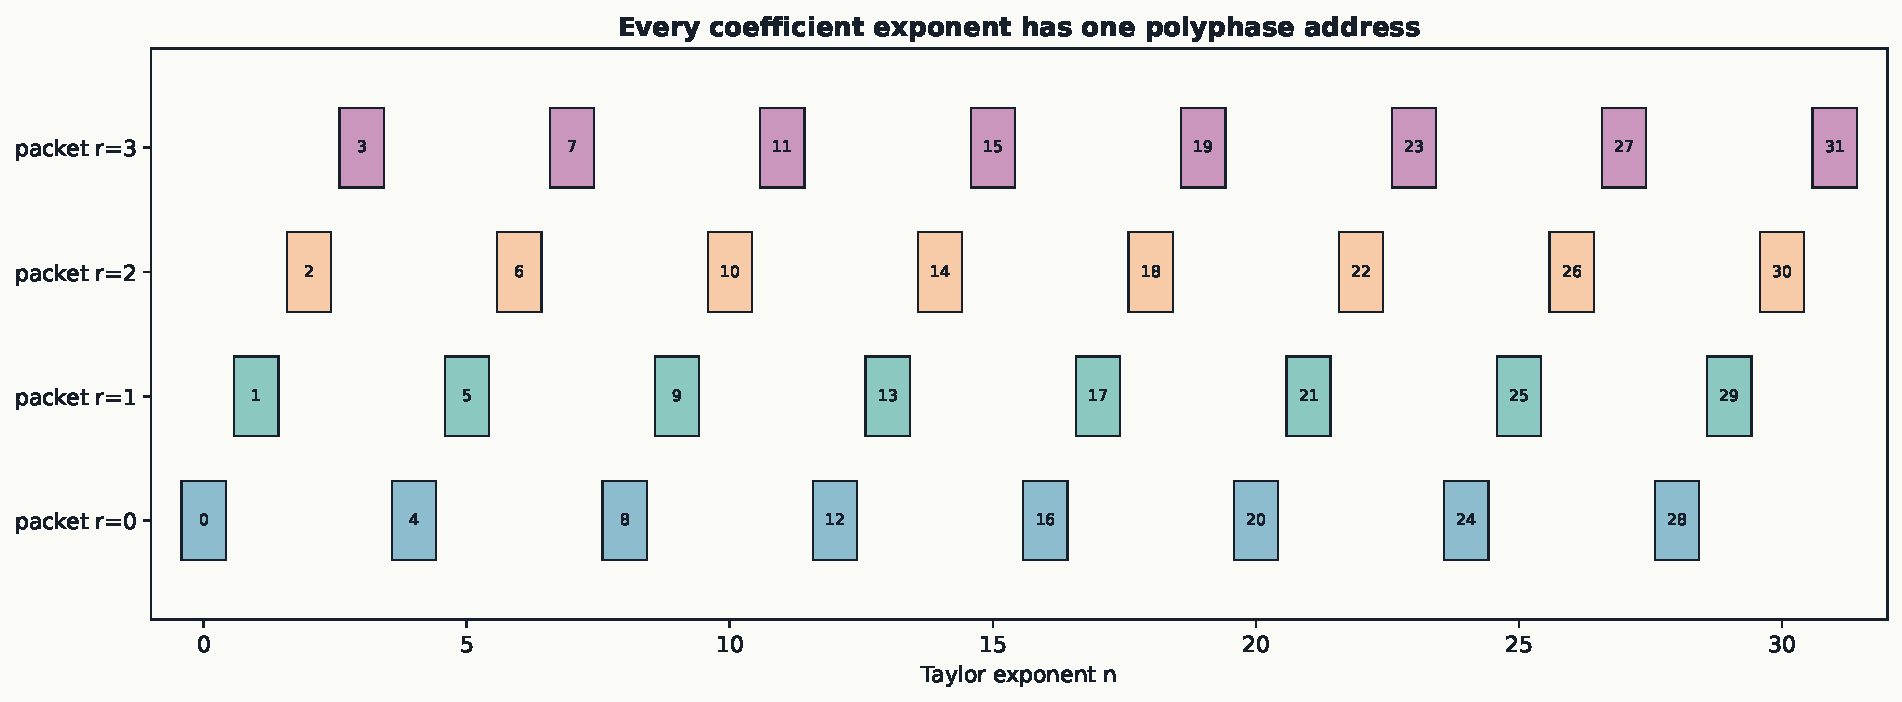
\includegraphics[width=\textwidth,height=0.60\textheight,keepaspectratio]{figures/I_01_polyphase_partition.pdf}
\caption{Residue addresses partition the coefficients and retain exact reconstruction. This is the algebraic entry point of Chapter 1. Source: Volume I, figure 01.}
\end{figure}
\clearpage
\section*{2. The arithmetic Gamma scale}
\addcontentsline{toc}{section}{2. The arithmetic Gamma scale}
\begin{figure}[H]
\centering
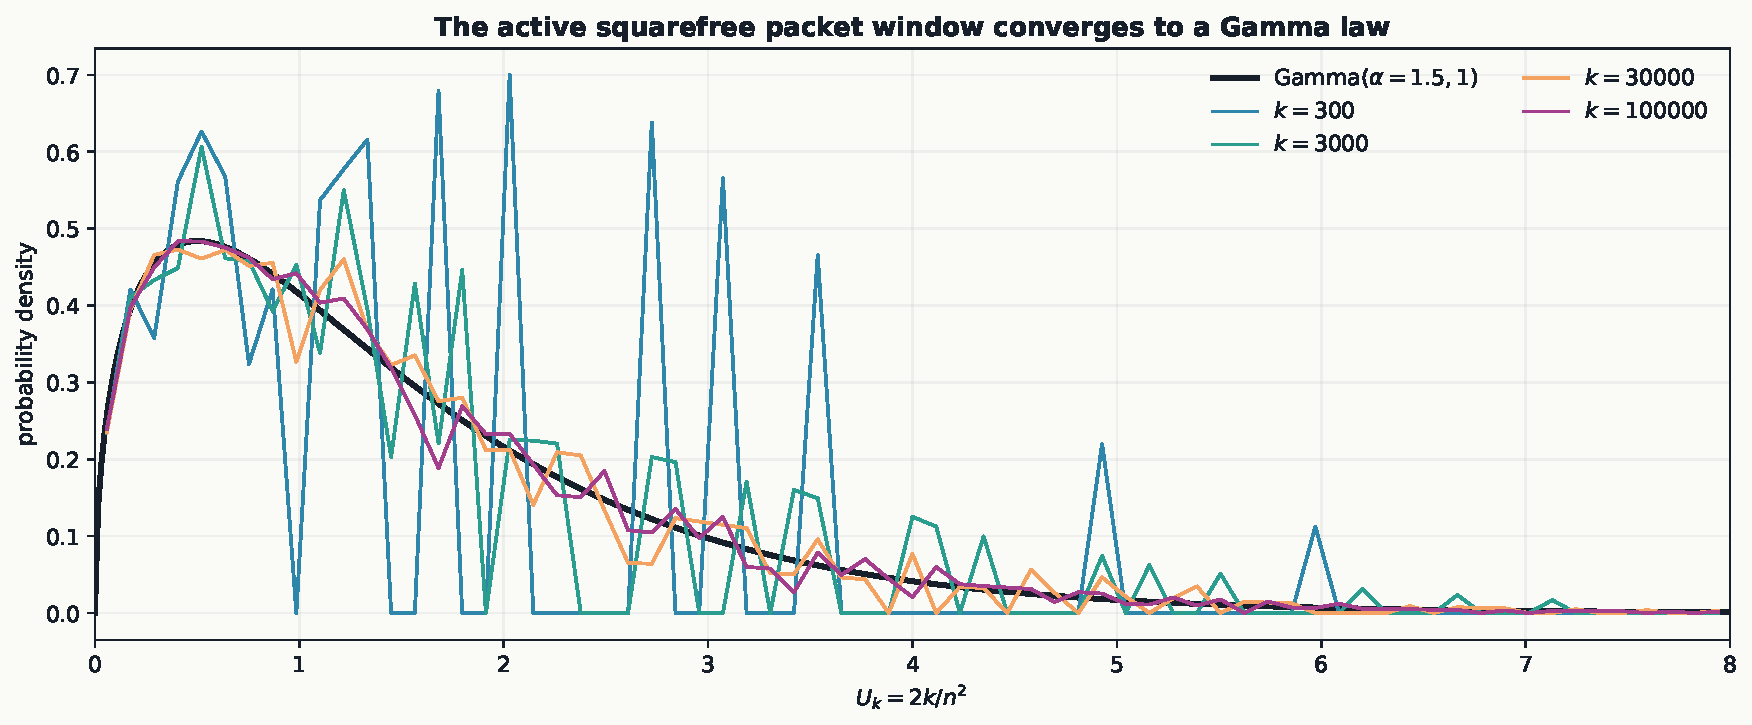
\includegraphics[width=\textwidth,height=0.60\textheight,keepaspectratio]{figures/II_14_gamma_scaling.pdf}
\caption{The finite-depth distributions approach the Gamma coordinate law. Chapter 1 separates the visual evidence from the all-moment proof. Source: Volume II, figure 14.}
\end{figure}
\clearpage
\section*{3. A common Laguerre fixed point}
\addcontentsline{toc}{section}{3. A common Laguerre fixed point}
\begin{figure}[H]
\centering
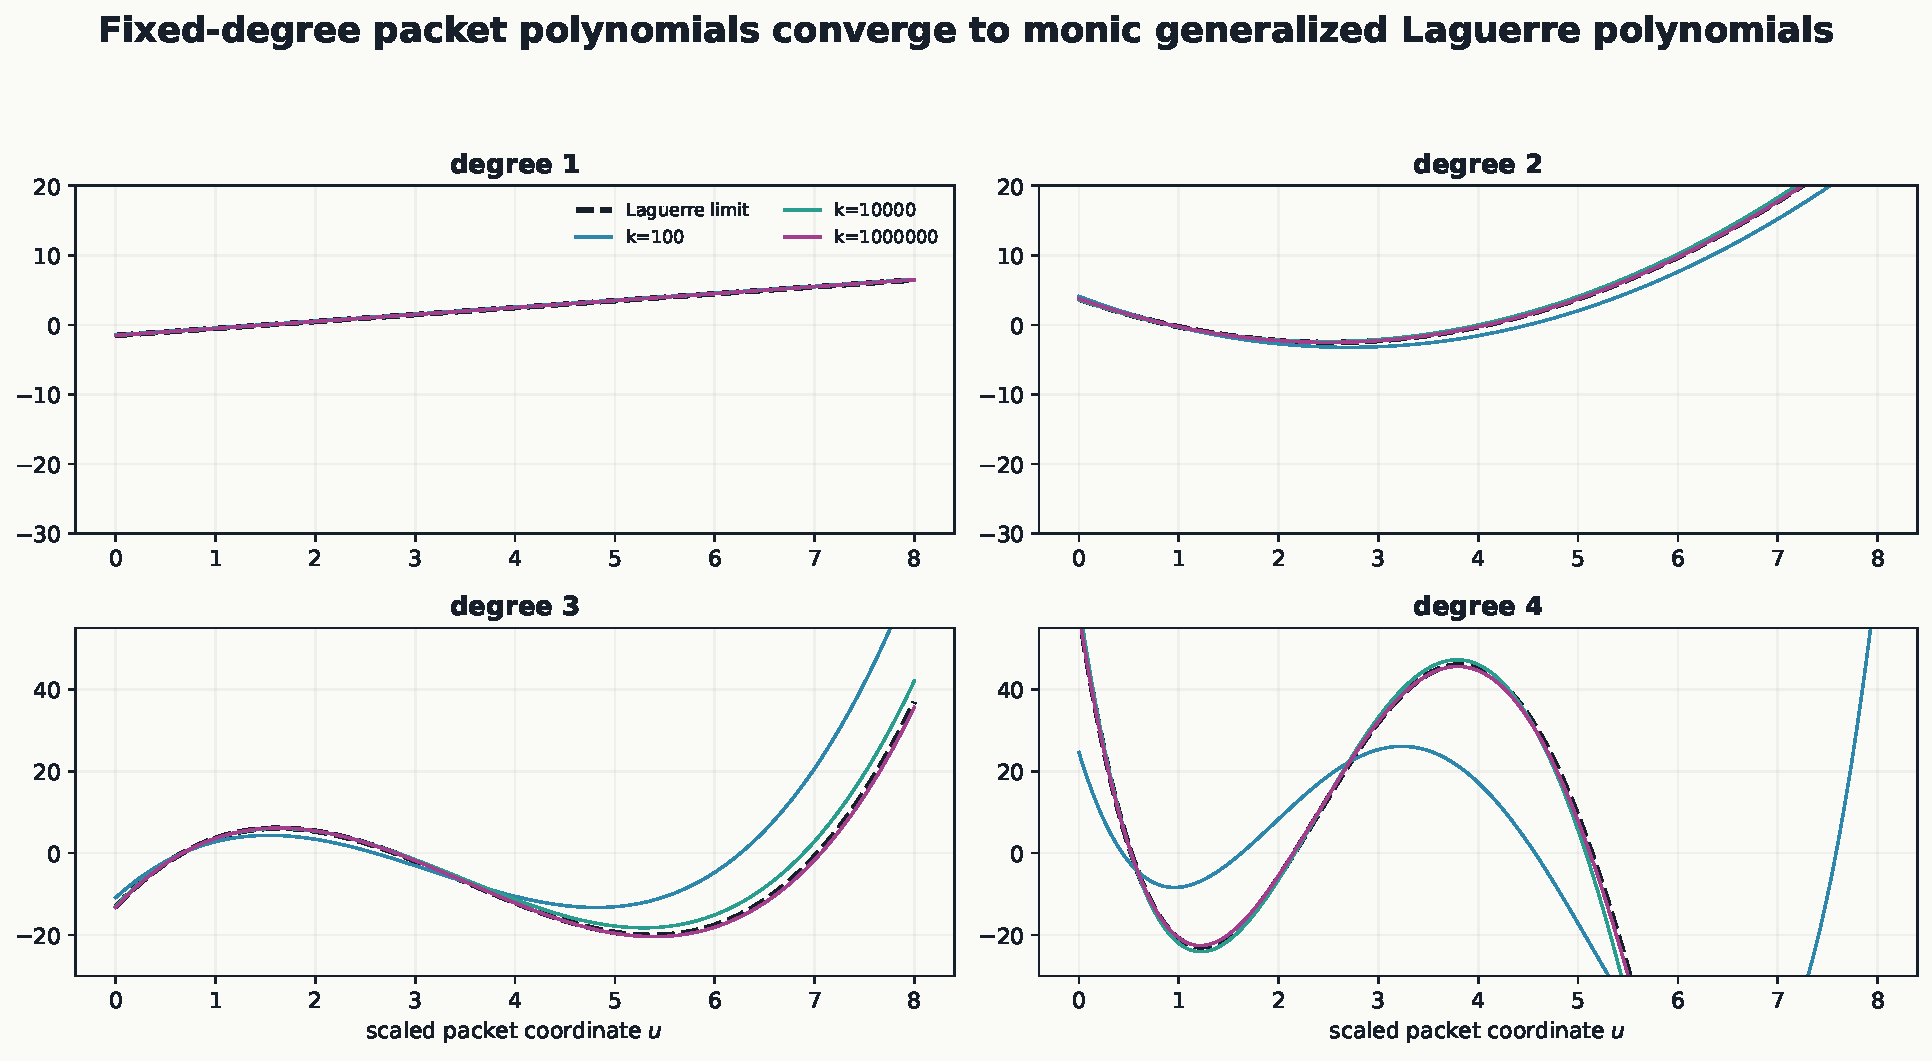
\includegraphics[width=\textwidth,height=0.60\textheight,keepaspectratio]{figures/III_13_laguerre_polynomial_limit.pdf}
\caption{Fixed-degree orthogonal polynomials converge after endpoint rescaling. The limiting moment matrix supplies the coefficient argument. Source: Volume III, figure 13.}
\end{figure}
\clearpage
\section*{4. The exact Gamma--sech window}
\addcontentsline{toc}{section}{4. The exact Gamma--sech window}
\begin{figure}[H]
\centering
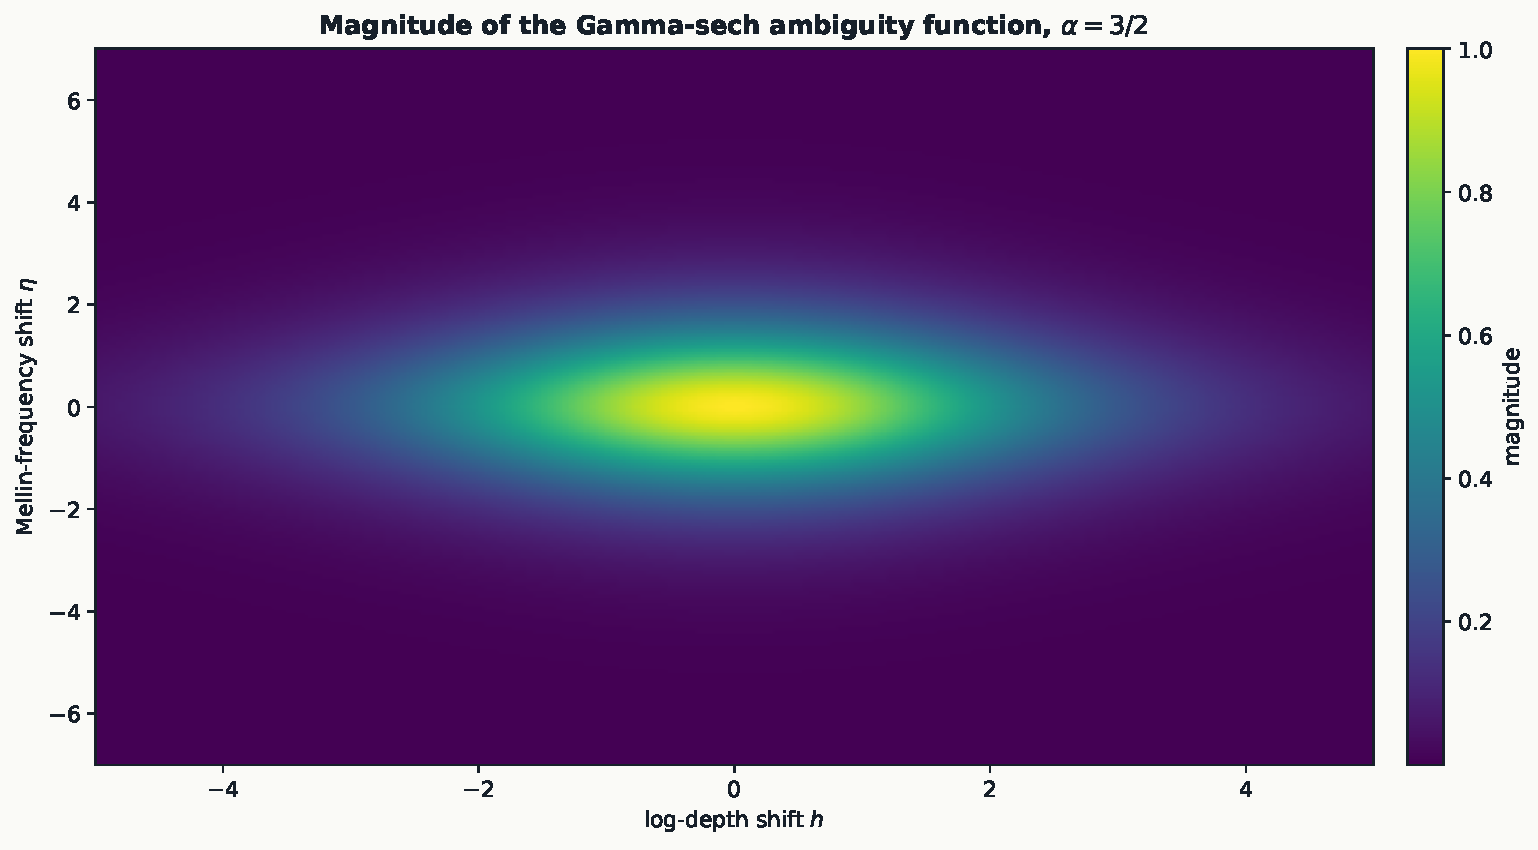
\includegraphics[width=\textwidth,height=0.60\textheight,keepaspectratio]{figures/V_06_ambiguity_magnitude.pdf}
\caption{The phase-space magnitude is generated from the normalized log-Gamma window. The corresponding cross-shape formula is proved in Chapter 2. Source: Volume V, figure 06.}
\end{figure}
\clearpage
\section*{5. Shape refinement}
\addcontentsline{toc}{section}{5. Shape refinement}
\begin{figure}[H]
\centering
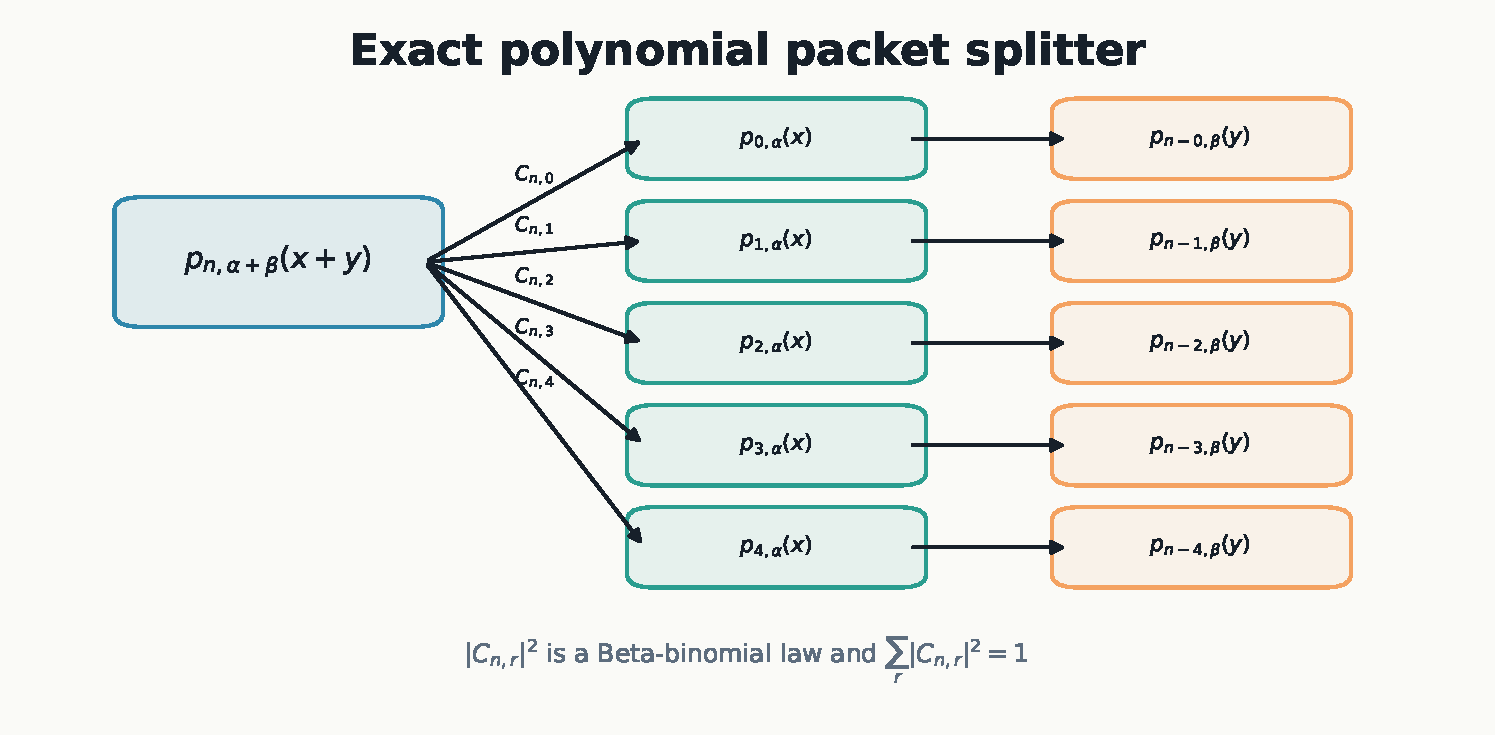
\includegraphics[width=\textwidth,height=0.60\textheight,keepaspectratio]{figures/VI_12_packet_splitter.pdf}
\caption{The normalized polynomial refinement distributes one total degree across two child shapes. Its squared coefficients form a beta-binomial law. Source: Volume VI, figure 12.}
\end{figure}
\clearpage
\section*{6. Finite recoupling}
\addcontentsline{toc}{section}{6. Finite recoupling}
\begin{figure}[H]
\centering
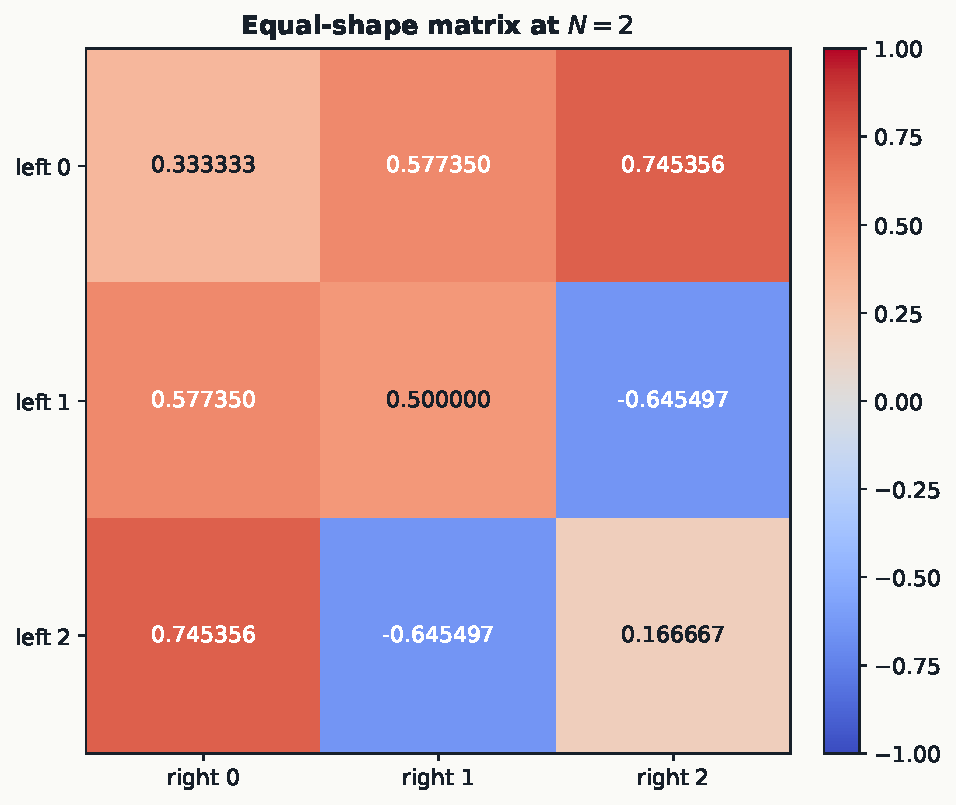
\includegraphics[width=\textwidth,height=0.60\textheight,keepaspectratio]{figures/VII_08_two_excitation_exact.pdf}
\caption{Signed amplitudes and their squared probabilities are different outputs of one finite transform. The gauge affects amplitude signs while preserving the measured kernel. Source: Volume VII, figure 08.}
\end{figure}
\clearpage
\section*{7. A deformable two-channel packet}
\addcontentsline{toc}{section}{7. A deformable two-channel packet}
\begin{figure}[H]
\centering
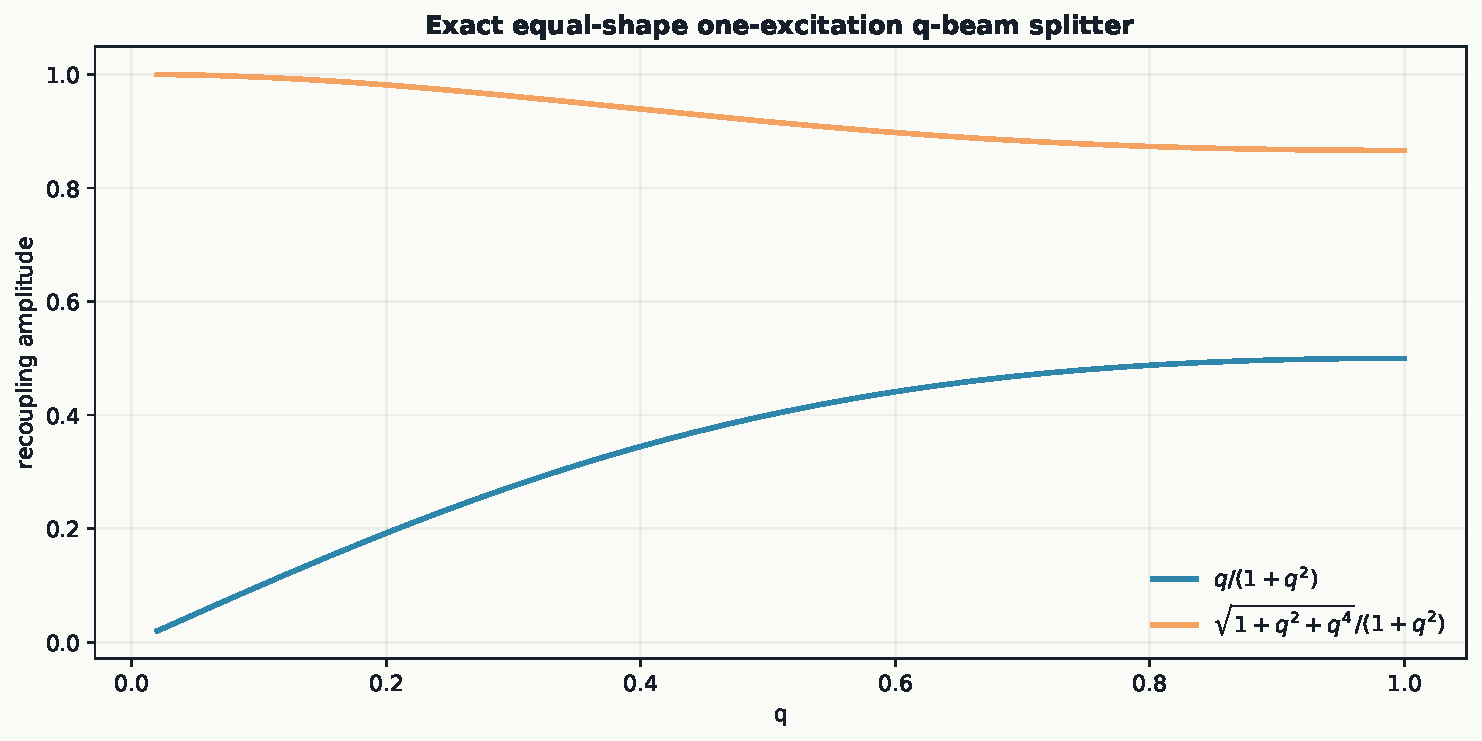
\includegraphics[width=\textwidth,height=0.60\textheight,keepaspectratio]{figures/VIII_07_q_beam_splitter_amplitudes.pdf}
\caption{The exactly derived one-excitation overlap connects classical mixing with a sparse routing limit. Higher-degree behavior requires its own analysis. Source: Volume VIII, figure 07.}
\end{figure}
\clearpage
\section*{8. A retained negative control}
\addcontentsline{toc}{section}{8. A retained negative control}
\begin{figure}[H]
\centering
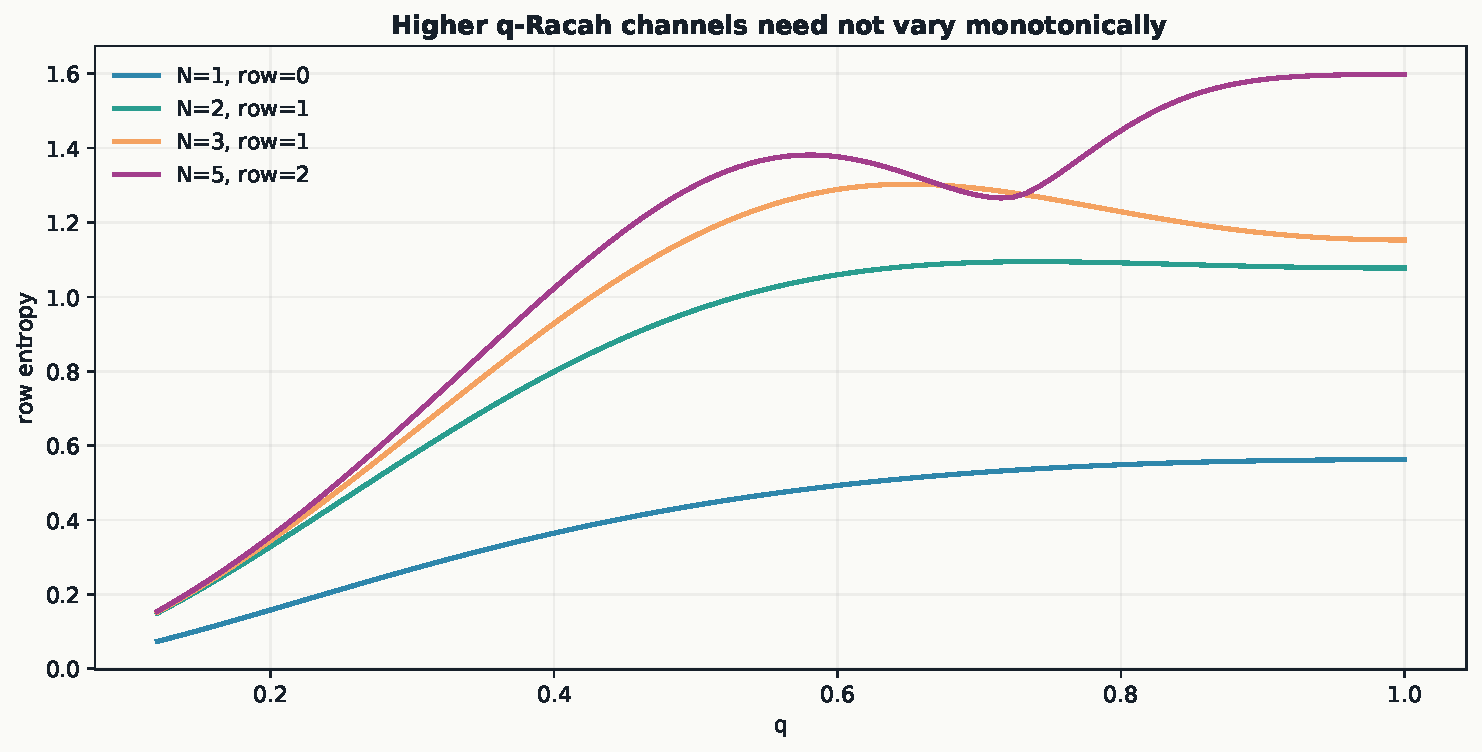
\includegraphics[width=\textwidth,height=0.60\textheight,keepaspectratio]{figures/VIII_21_entropy_nonmonotonicity.pdf}
\caption{The source figure exhibits a higher-excitation entropy decrement as q varies. Fixed-kernel entropy nondecrease after measurement does not imply monotonicity along deformation. Source: Volume VIII, figure 21.}
\end{figure}

\chapter{Corrections and proof dependencies}

The following register governs the preserved source papers in the complete reader. It separates false wording, missing hypotheses, and incomplete proof implications. The review was bounded to the current I--VIII manuscripts and selected decisive checks; it does not certify every theorem. The full review notes retain exact source locators.

\section{Endpoint and character conventions}

\textbf{C01 / Volume II, Proposition 13.1: zero depth.}
The number-basis matrix element on $\ell^2(\{2,3,\ldots\})$ omits the $n=1$ term at $k=0$. Its contribution is one under the moment convention $0^0=1$. State the displayed identities for $k\ge1$, or retain the separate zero-eigenvalue atom of the positive contraction. The logarithmic scale generator is used only on $n\ge2$. This is a correction after a stated restriction, not a failure of the positive measure.

\textbf{C02 / Volumes III--V: modulus and conductor.}
For a character modulo $q$, $|\chi(n)|^2=\boldsymbol 1_{(n,q)=1}$. An induced character can have a smaller conductor without changing its actual zero set. The principal character modulo four has conductor one but vanishes at two. Thus the coprimality parameter and squarefree density use the modulus; a conductor formulation requires the character to be primitive modulo that conductor. The consolidated chapters use the modulus convention.

\textbf{C03 / Volume I, Chapter 14: wavelet mean.}
The zero-integral Mertens-wavelet sentence requires $k\ge1$. At $k=0$, its stated integral is one. The subsequent source Mellin theorem already has the needed positive-depth restriction.

\section{Positive spectral models}

\textbf{C04 / Volume III, abstract and claim map: quadrature support.}
Gaussian quadrature nodes lie in the interval spanned by a positive measure; they need not be original discrete spectral points. For $a=\beta=2$, $q=1$, and one quadrature node, the node is $E_1/E_0$. The original spectrum has zero and its first positive point $9/16$. Directly,
\[
0<\frac{E_1}{E_0}<\sum_{n\ge2}n^{-4}
<\frac1{16}+\int_2^\infty x^{-4}\,dx
=\frac5{48}<\frac9{16}.
\]
The node lies in the spectral gap. The actual moment-exact theorem survives this correction. Exact Gaussian nodes here are in $(0,1)$; a tiny floating-point node is not an exact representation of the atom at zero.

\textbf{C05 / Volume III, Corollary 5.2: residue sign.}
The weights in $E_0\lambda_j/(1-z\xi_j)$ are positive. The complex residue at $z=1/\xi_j$ is
\[
\operatorname*{Res}_{z=1/\xi_j}
\frac{E_0\lambda_j}{1-z\xi_j}
=-\frac{E_0\lambda_j}{\xi_j}<0.
\]
The corrected statement is ``positive spectral weights and poles on $(1,\infty)$.''

\textbf{C06 / Volume III, Theorems 6.1--7.1: all moments.}
Weak convergence against bounded continuous functions does not by itself imply convergence of polynomial moments. Chapter 1 supplies the missing implication from Volume II's shifted-energy identity. It also transfers the moments between $U_k=2k n^{-\beta}$ and $u_k=U_k-U_k^2/(4k)$. This closes the proof linkage needed for the fixed-degree Laguerre and determinant arguments.

\textbf{C07 / Volume III, Theorem 11.1: endpoint cusp.}
The original proof informally replaces a discrete measure by a density. Chapter 1 supplies an Abelian proof directly from $E_k\sim A k^{-3/2}$, with no density replacement. The resulting coefficient is the stated $3/(2^{3/2}\pi)$. This repairs the local proof passage conditional on the source energy law and its counting input. It does not provide a new signed arithmetic estimate.

\section{Signed rational models}

\textbf{C08 / Volume IV, Theorem 11.1: denominator degree.}
Hankel nonbreakdown establishes unique normalized rational matching with $\deg P\le m-1$ and $\deg Q\le m$. An ordinary $m$-term simple-packet decomposition additionally follows when $\deg Q=m$ and its $m$ zeros are simple. The source proof does not establish that full-degree implication for every arithmetic packet.

Generic signed moments $(0,1,0,0)$ at $m=2$ have a nonzero Hankel determinant but matching rational function $z$ and denominator one. This illustrates the missing general implication; it is not a counterexample within the M\"obius arithmetic family. Preserve the rational matching result and qualify its simple-packet extension. Positivity, real support, and universal numerical stability are not implied.

\section{Recoupling and deformation}

\textbf{C09 / Volume VII, finite recurrence: sign gauge.}
An irreducible real tridiagonal matrix has nonzero signed off-diagonal entries. Positive entries require a diagonal sign gauge. For the displayed equal-half-shape one-excitation matrix,
\[
R=\begin{pmatrix}1/2&\sqrt3/2\\\sqrt3/2&-1/2\end{pmatrix},
\qquad R\operatorname{diag}(0,2)R^T
=\begin{pmatrix}3/2&-\sqrt3/2\\-\sqrt3/2&1/2\end{pmatrix}.
\]
The displayed matrix therefore cannot satisfy the asserted positive-off-diagonal recurrence in that same gauge. Chapter 3 states the gauge transformation explicitly.

\textbf{C10 / Volumes VII--VIII, pentagon interpretation.}
The product of overlap matrices telescopes for any complete orthonormal bases of one common space. Consistent sign changes, permutations, or a shared incorrect subspace can still give identity. The theorem is valid; the inference that every wrong phase, ordering, or projector must be detected by closure is false. Representation relations, lowest-weight annihilation, pair spectra, and tree eigen-equations must be checked separately. A small closure residual is one consistency check.

\textbf{C11 / Volume VIII, scalar q-Racah family.}
Termination through a denominator parameter $q^{-N}$ alone does not guarantee a positive orthogonal family. Let $N=1$, $q=1/2$, and
\[
\alpha=\beta=1/2,\qquad\gamma=4,\qquad\delta=1.
\]
Then $\gamma q=q^{-N}=2$, all terms needed for $n,y\in\{0,1\}$ have nonzero denominators, yet the two lattice values coincide:
\[
\mu(0)=\mu(1)=3,\qquad R_0=(1,1),\quad R_1=(1,1).
\]
Nondegenerate lattice and admissible positive-weight hypotheses are necessary. Chapter 3 distinguishes a well-defined terminating scalar formula from an orthogonal family.

\textbf{C12 / Volume VIII: scalar-to-matrix comparison.}
The implemented positive Casimir-overlap matrix and the standalone scalar q-Racah fixture are separate constructions. Duality and classical-limit checks of the latter do not establish equality with the former. The exact parameter dictionary, weight normalization, and phase convention remain a comparison obligation. Generic Askey--Wilson eigenfunction identities likewise do not confer positive orthogonality without parameter hypotheses.

\section{Retained open statements and review limits}

The principal M\"obius coherence estimate remains open. Its three ledger conjecture entries are provenance for one recurring target, not three independent conjectures. The higher-excitation q-entropy monotonicity claim is excluded by Volume VIII's own negative control; fixed-kernel entropy nondecrease after measurement remains valid.

Classical recoupling/tridiagonal identifications, strong Schwartz convergence in the heat limit, and full bibliography normalization were not all rederived in this consolidation. Their source dependencies remain explicit. The supplied elementary repairs were self-reviewed; the cusp lemma also received a separate neutral subagent audit. Agreement between reviewers is not a kernel certificate.

\chapter{Source crosswalk and evidence}

\section{The consolidation map}

\begin{longtable}{L{0.12\textwidth}L{0.24\textwidth}L{0.54\textwidth}}
\toprule
Sources & Shared block & Retained mathematical work\\
\midrule
\endhead
I--IV & Arithmetic packets & Coefficient and Bernoulli refinement; cyclotomic germs and invariants; reciprocal L-value transfers; positive squarefree measure, moments, resolvent, finite Jacobi models, Gamma/Laguerre scaling; signed continuation.\\
IV--VI & Shape packets & Depth-time Gram lift; joint Gamma--sech limit; exact log-Gamma window; Fourier/Wigner coordinates; orthogonal bases; shape convolution, refinement, transfers, coherent smoothing.\\
VI--VIII & Recoupling & Positive discrete-series ladder; lowest-weight projectors; Casimir atlases; ordinary and q-deformed overlaps; measurement kernels; deformation generator; pentagon and finite compilation.\\
I, II, V & Open arithmetic boundary & One principal signed coherence target, retaining the three original conjecture-record links.\\
\bottomrule
\end{longtable}

This manuscript selects a mathematical spine rather than reproducing every invariant or example. Volume I's Wronskian negative control, Volume II's Stieltjes/resultant details, the full Wigner formulas in V, and the complete transfer/frame estimates in VI remain available in the preserved papers. The source crosswalk groups related material; it does not certify that differently stated claims are equivalent or count distinct results.

The eight originals contain 431 PDF pages. The source package also preserves the earlier special-function registry as context. It is not silently merged with the numbered series. The complete reader's machine-readable index gives each paper's physical page range, which differs from its original printed page labels.

\section{Fresh test run}

\begin{center}
\begin{tabular}{lrrr}
\toprule
Volume & Fresh pytest passed & Archived built-in passed & Source PDF pages\\
\midrule
I & 13 & 51 & 60\\
II & 18 & 61 & 50\\
III & 19 & 34 & 38\\
IV & 18 & 18 & 55\\
V & 19 & 19 & 52\\
VI & 21 & 24 & 54\\
VII & 20 & 13 & 60\\
VIII & 20 & 23 & 62\\
\midrule
Total & 148 & 243 & 431\\
\bottomrule
\end{tabular}
\end{center}

All 148 collected pytest cases passed, with zero failures, errors, or skips. Each suite ran from a clean temporary source copy. SHA256 comparisons confirmed that the original extracted source trees remained unchanged. Tests include recomputed numerical and symbolic identities as well as archival-ledger, figure, and manuscript checks.

The archived built-in ledgers report 243 successful checks. Only the 64 built-in checks in Papers I and VII were recomputed by the current pytest run. The remaining built-in totals are historical records. Neither test count is a universal proof count. The JSON report preserves exact commands, environment versions, timings, and case-level results. Small exact correction witnesses are recorded separately.

\section{Formalization scope}

The retrieved projector-calculus ledger has 173 special-function source objects: 125 theorem, proposition, lemma, or corollary records; 15 definitions; 22 context, example, or algorithm records; eight boundary records; and three conjecture records.

\begin{center}
\begin{tabular}{lrr}
\toprule
Volume & Source objects & Theorem/lemma/proposition/corollary records\\
\midrule
I & 32 & 22\\
II & 23 & 15\\
III & 24 & 16\\
IV & 16 & 10\\
V & 21 & 17\\
VI & 22 & 20\\
VII & 15 & 10\\
VIII & 20 & 15\\
\midrule
Total & 173 & 125\\
\bottomrule
\end{tabular}
\end{center}

The statuses are 88 phase-1-queued, 51 queued, one Lean-draft-present, 22 context/example, eight boundary, and three conjectural. No special-function claim in that retrieved ledger has a kernel-checked source-claim status. The actual special-function Lean tranche inspected contains one coefficient-subsequence refinement theorem. It does not formalize the complete analytic series, Gamma limits, orthogonal-polynomial analysis, or signed coherence estimate.

The whole-project v1.1.0 static figures of 594 claim records and 104 theorem-like Lean declarations are not special-function proof counts. That release explicitly reports that a kernel build was not attempted. The later finite browser-safe core does not establish analytic completion of this series. These findings are bounded by the targeted files and searches recorded in the scope report.

\section{Primary-source checks}

The following exact external inputs received bounded primary-source checks in this edition. Other source-paper bibliographies remain preserved for subsequent normalization.

\begin{enumerate}[leftmargin=*]
\item L. B\'aez-Duarte, \emph{A sequential Riesz-like criterion for the Riemann hypothesis}, International Journal of Mathematics and Mathematical Sciences 2005, 3527--3537, Theorem 1.1. DOI: \href{https://doi.org/10.1155/IJMMS.2005.3527}{10.1155/IJMMS.2005.3527}. Its binomial coefficients agree with Chapter 1's $c_k$ by the exact reciprocal-zeta identity; its arbitrary-positive-exponent bound gives the stated coherence equivalence.
\item NIST DLMF, \href{https://dlmf.nist.gov/18.28}{Section 18.28}, equations 18.28.1\_5 and 18.28.6\_1--6\_2. These match the normalized scalar Askey--Wilson function and the q-difference operator in VIII. The separate orthogonality parameter restrictions are not inferred from the eigenfunction identity.
\item W. Gautschi, \emph{Orthogonal polynomials: applications and computation}, Acta Numerica 5 (1996), 45--119, opening Gaussian-quadrature discussion and support-interval statements. The quadrature support is an interval containing the measure's support, not an assertion that quadrature nodes are original atoms. The decisive counterexample in Chapter 5 is proved directly from the packet measure.
\end{enumerate}

The accompanying literature notes state exactly what was checked and what was not. The consolidation makes no global novelty claim. Classical special functions retain their established names; the unified organization records how reconstruction, refinement, positive models, shape transfer, and recoupling are composed within the packet calculus.

\end{document}
